\PassOptionsToPackage{quiet}{fontspec}
\documentclass[12pt,a4paper,UTF8]{article}
\usepackage{thesis} % 格式控制
\usepackage{indentfirst}
\usepackage{amsmath} % 数学公式支持
\usepackage{amsfonts} % 数学字体支持
\usepackage{amssymb} % 数学符号支持
\usepackage{graphicx} % 图片插入支持
\usepackage{float} % 浮动体位置控制，支持 [H] 选项
\usepackage{caption} % 图表标题格式控制
\usepackage{geometry} % 页面布局控制
\usepackage{setspace} % 行距控制
\usepackage{xeCJK} % 中文字体支持
\usepackage{fontspec} % 字体设置
\usepackage[most]{tcolorbox} % 高亮按键命令
\setlength{\parindent}{2em} % 控制首行缩进  
\addtolength{\parskip}{3pt} % 控制段落距离  
\onehalfspacing % 1.5倍行距  
\graphicspath{{./figures/}} % 指定图片所在文件夹  
\setCJKmainfont{SimSun}
% 定义中文字体命令
\setCJKfamilyfont{hei}{SimHei} 

\classname{天线理论与设计}  % 设置课程名称
\makepagestyle{}{\printclassname ~实验报告}

% 自定义命令
\newtcbox{\keyblue}{on line,
  colframe=blue!60!black, colback=blue!10,
  boxrule=0.8pt, arc=2pt, boxsep=0pt, left=2pt, right=2pt, top=1pt, bottom=1pt,
  tcbox raise base, fontupper=\color{blue}\bfseries}

\begin{document}
\maketitlepage{HFSS单极子天线仿真}{玉泉教4-302}{郑智瑄}{3230103913}{\today}{王浩刚} %封面页 

\maketoc    %目录页

\section{\heiti\bfseries 实验背景与目的}
\begin{itemize}
    \item {\heiti\bfseries 背景}：半波偶极子天线作为一种经典的对称阵子天线，广泛应用于通信、雷达、导航等领域。
随着无线通信技术的快速发展，对天线性能的要求也日益提高，因此，通过HFSS（
High Frequency Structure Simulator）等仿真工具对天线进行精确设计和优化显得
尤为重要。
    \item {\heiti\bfseries 目的}：本设计旨在利用HFSS仿真软件，对半波偶极子天线进行详细的建模、仿真和分析，以
了解其辐射特性、阻抗匹配、驻波比等关键参数，为实际工程应用提供理论依据和技术
支持。同时，通过本设计实践，加深对HFSS软件使用方法的理解，掌握天线设计与仿
真的基本流程和方法。
\end{itemize}

\section{\heiti\bfseries 设计任务与要求}
\begin{itemize}
    \item {\heiti\bfseries 设计任务}：设计一个中心频率为3GHz的半波偶极子天线，包括天线模型的建立、边界条件的设置、激励方式的选择、求解参数的设置等。

    \item {\heiti\bfseries 设计要求}：天线应具有良好的辐射特性，如较宽的辐射带宽、稳定的辐射方向图等；同时，天线的阻抗匹配应良好，以确保信号的有效传输。此外，设计过程中需充分考虑天线的实际应用场景，如安装环境、馈电方式等因素对天线性能的影响。
\end{itemize}

\section{\heiti\bfseries 半波偶极子天线原理}
\subsection{\heiti\bfseries 电流分布}
\begin{itemize}
    \item 对于从中心馈电的偶极子，其两端开路，故电流为零。
工程上通常将其电流分布近似为正弦分布
    \item 假设天线沿z轴放置，其中心坐标位于坐标原点，如图
所示，则长度为l的偶极子天线的电流分布为：
\begin{equation}
I(z) = I_m \sin\left(\frac{\pi}{2} - kz\right) = I_m \cos(kz)
\end{equation}
其中，$I_m$为最大电流幅度，$k = 2\pi/\lambda$为波数，$z$为沿天线轴向的坐标。

\begin{figure}[H]
    \centering
    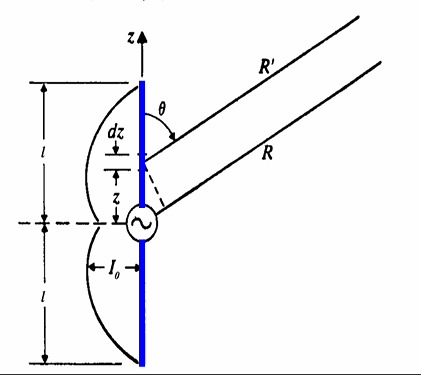
\includegraphics[width=0.8\textwidth]{fig1.png}
    \caption{半波偶极子天线电流分布示意图}
\end{figure}

\end{itemize}
\subsection{\heiti\bfseries 辐射场与方向图}
已知半波偶极子天线上的电流分布，可以利用叠加原理计算其辐射场，有：
\begin{equation}
E = j\frac{60I_m}{r} \frac{\cos\left(\frac{\pi}{2}\cos\theta\right)}{\sin\theta} e^{-jkr}\hat{e}_\theta = j\frac{6I_m m}{r} f(\theta,\phi)\hat{e}_\theta
\end{equation}

其中半波偶极子天线的方向性函数为：
\begin{equation}
f(\theta,\phi) = f(\theta) = \frac{\cos\left(\frac{\pi}{2}\cos\theta\right)}{\sin\theta}
\end{equation}

\subsection{\heiti\bfseries 方向性系数}
根据公式可计算出半波偶极子天线的方向性系数为：
\begin{equation}
D = \frac{1}{\frac{1}{4\pi}\int_0^{2\pi}\int_0^{\pi}\frac{\cos^2\left(\frac{\pi}{2}\cos\theta\right)}{\sin^2\theta}\sin\theta d\theta d\phi} = 1.64 = 2.15dB
\end{equation}

\subsection{\heiti\bfseries 辐射电阻}
天线的平均功率密度可以用平均坡印廷矢量来表示：
\begin{equation}
P_{av} = \frac{1}{2}(E \times H^*) = \frac{15I_m^2}{\pi r^2} \left(\frac{\cos\left(\frac{\pi}{2}\cos\theta\right)}{\sin\theta}\right)^2
\end{equation}

半波偶极子天线的辐射功率为：
\begin{equation}
P_r = \int P_{av}dS = \int_0^{2\pi} \int_0^{\pi} \frac{15I_m^2}{\pi r^2} \left|\frac{\cos\left(\frac{\pi}{2}\cos\theta\right)}{\sin\theta}\right|^2 r^2 \sin\theta d\theta d\phi = 36.6I_m^2
\end{equation}

用$R_r$表示辐射电阻，有：
\begin{equation}
P_r = 36.6I_m^2 = 0.5I_m^2 R_r
\end{equation}

求得：
\begin{equation}
R_r = 73.2\Omega
\end{equation}

\subsection{\heiti\bfseries 输入阻抗}
对于半波偶极子天线而言，输入阻抗近似看为辐射电阻73.2Ω。可见，半波偶极子天线的输入阻抗是纯电阻，易于和馈线匹配，这也是它被较多采用的原因之一。
\clearpage
\section{\heiti\bfseries 半波偶极子天线设计与仿真}
\subsection{\heiti\bfseries 新建设计工程}

（1）运行\keyblue{Ansys Electronics Desktop Student}并新建 HFSS 工程，重命名为 dipole；

（2）设置求解类型：在菜单栏中选择\keyblue{HFSS}—\keyblue{Solution Type}，在弹出窗口中选择\keyblue{Modal}，完成设置；

（3）设置模型长度单位：在主菜单栏中选择\keyblue{Modeler}-\keyblue{Units}，选择\keyblue{mm}。
\begin{figure}[H]
        \centering
        \begin{minipage}[b]{0.5\linewidth}
            \centering
            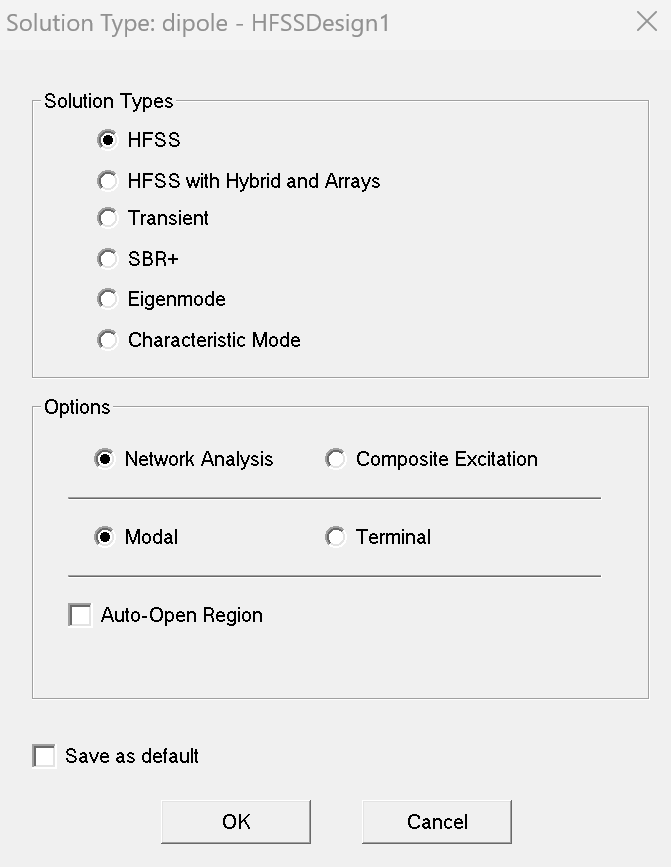
\includegraphics[width=0.9\textwidth]{p1.png}
            \caption{设置求解类型}
             
        \end{minipage}%
        \begin{minipage}[b]{0.5\linewidth}
            \centering
            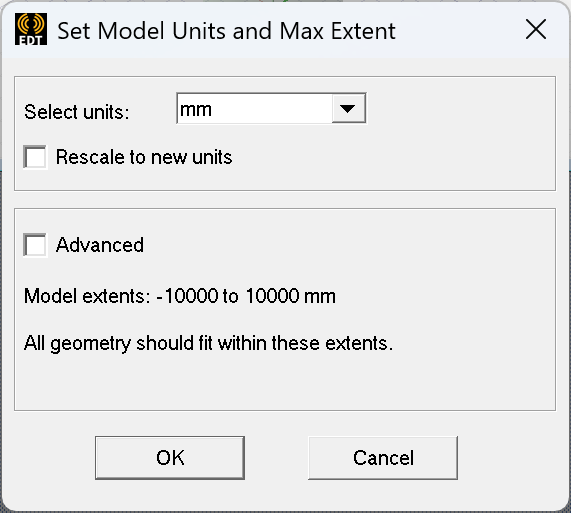
\includegraphics[width=0.9\textwidth]{p2.png}
            \caption{设置模型长度单位}
             
        \end{minipage}
    \end{figure}

    
\subsection{\heiti\bfseries 添加和定义设计变量}

在主菜单栏中选择\keyblue{HFSS}—\keyblue{Design Properties}，打开设计属性对话框，单击\keyblue{Add}按钮，打开\keyblue{Add Property}对话框，依次定义变量，如下图所示：

\begin{figure}[H]
    \centering
    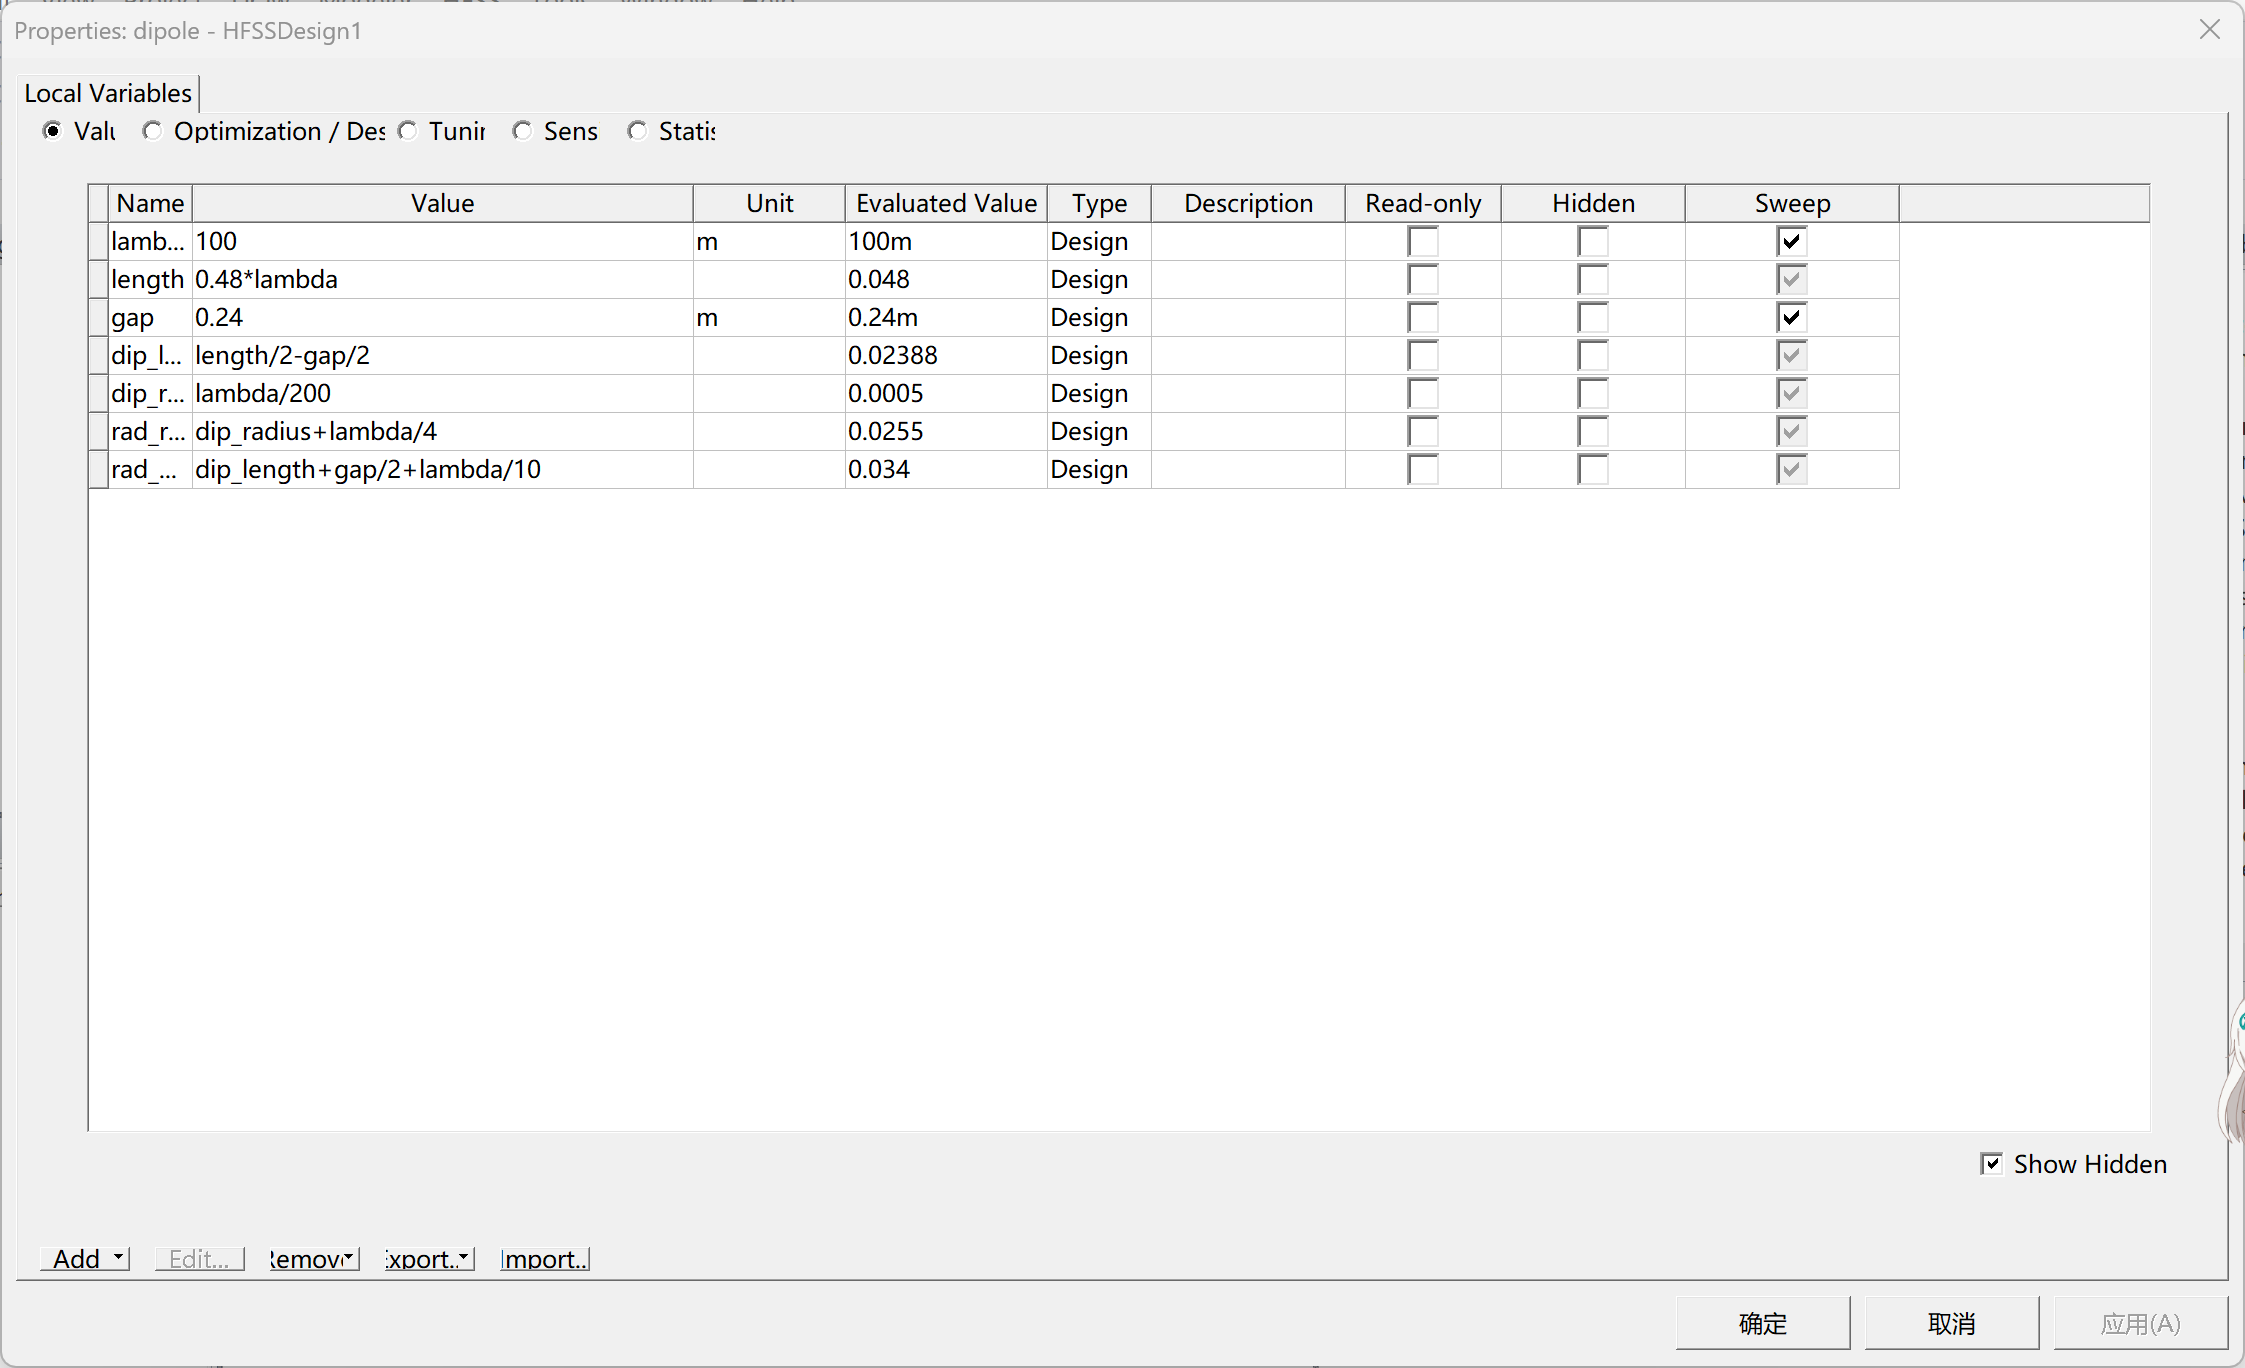
\includegraphics[width=0.8\textwidth]{p3.png}
    \caption{添加和定义设计变量}
\end{figure}

\subsection{\heiti\bfseries 设计建模}
\subsubsection{\heiti\bfseries 创建偶极子天线模型}

（1）在主菜单栏中选择\keyblue{draw}----\keyblue{cylinder}创建圆柱体，圆柱体名称设置为 Dipole，其材质为\keyblue{pec}；

\begin{figure}[H]
    \centering
    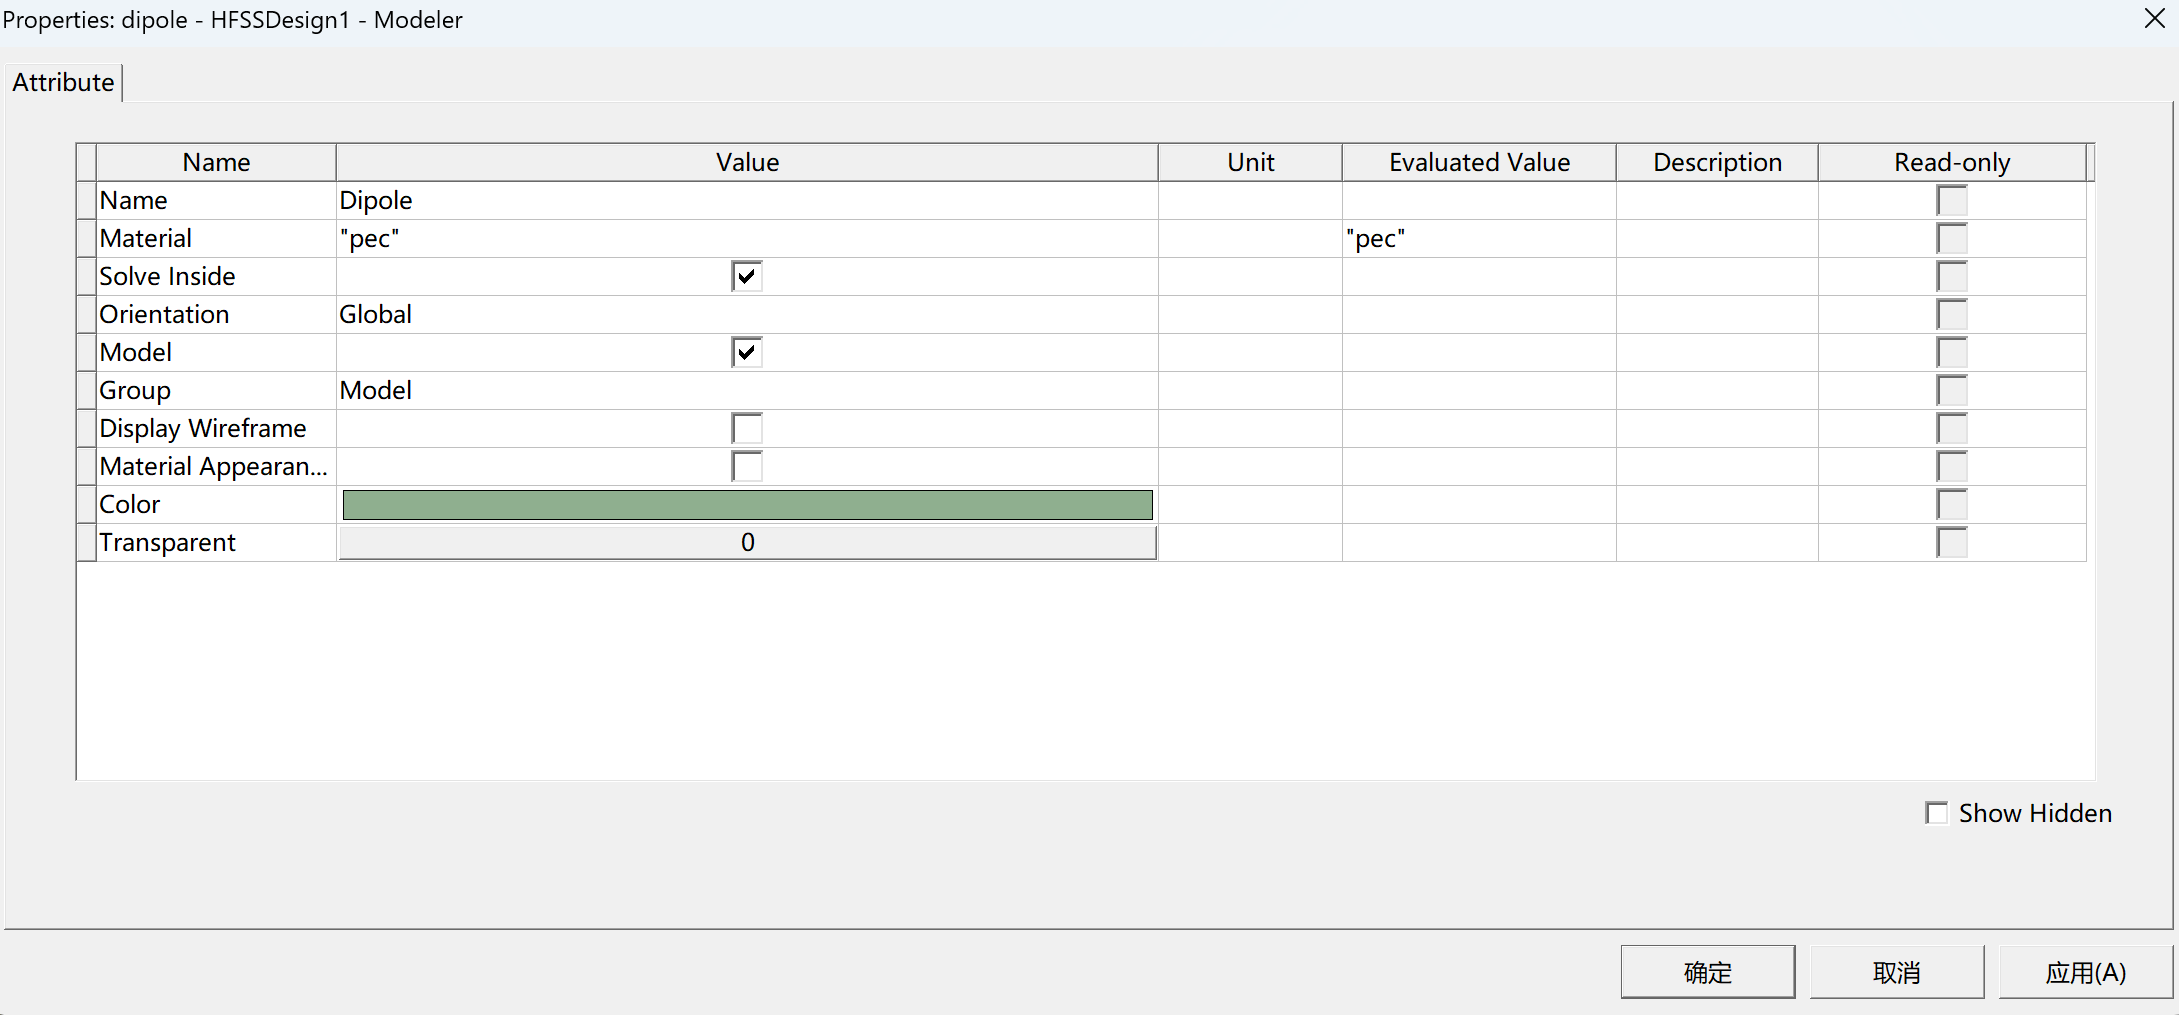
\includegraphics[width=0.8\textwidth]{p4.png}
    \caption{辐射边界圆柱体设置}
\end{figure}

（2）双击操作历史树中的\keyblue{Dipole}----\keyblue{createcylinder}节点，打开新建圆柱体属性对话框的\keyblue{command}选项卡，在该选项卡中设置圆柱体的底面圆心坐标、半径和长度，如下所示：

\begin{figure}[H]
    \centering
    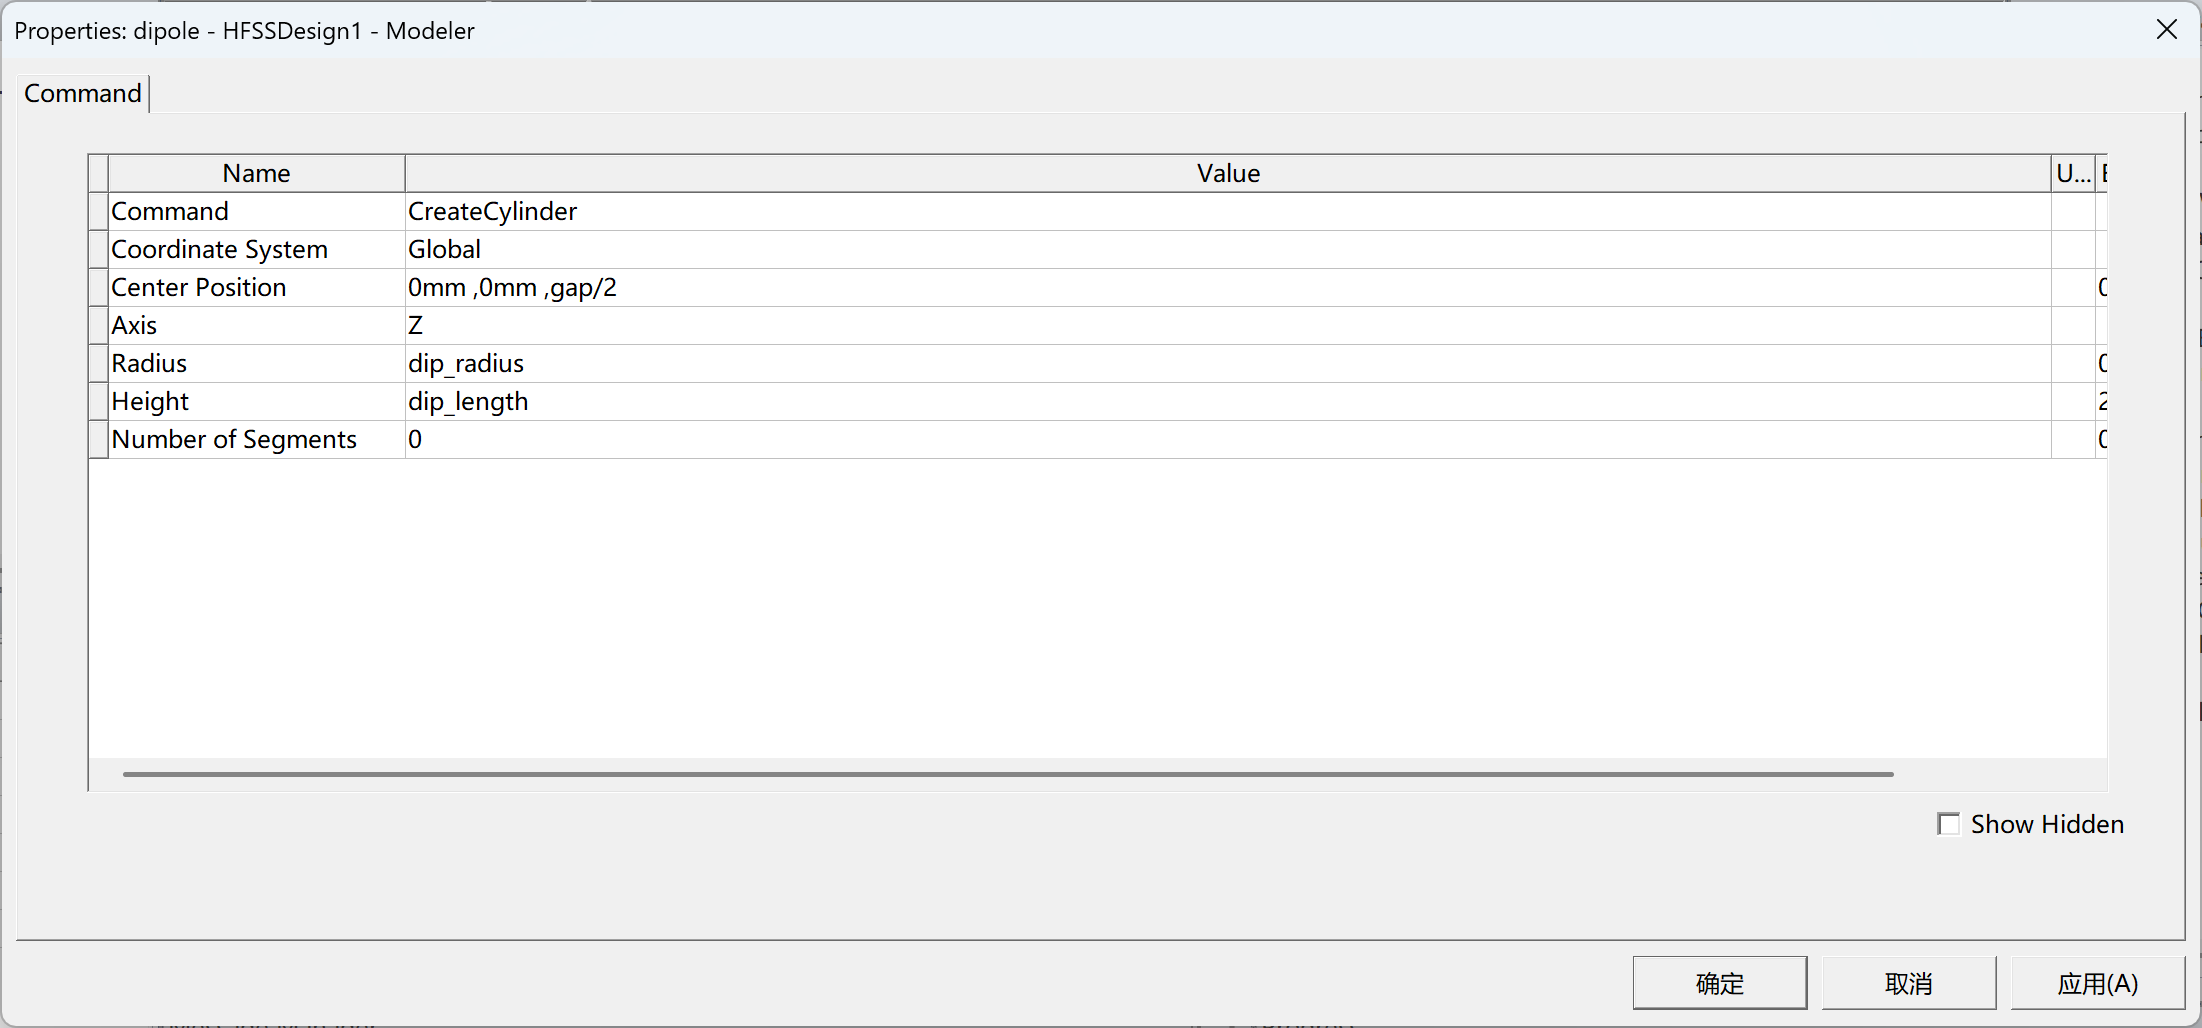
\includegraphics[width=0.8\textwidth]{p5.png}
    \caption{辐射边界圆柱体设置}
\end{figure}

（3）选中创建的圆柱体模型，然后从主菜单中选择\keyblue{Edit}–\keyblue{Duplicate}–\keyblue{Around}–\keyblue{Axis}，执行沿坐标轴的复制。在打开的对话框中进行如下设置：

\begin{figure}[H]
    \centering
    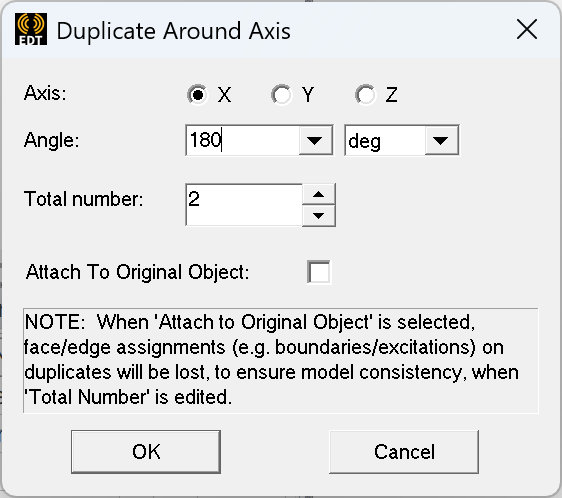
\includegraphics[width=0.8\textwidth]{p7.png}
    \caption{辐射边界圆柱体设置}
\end{figure}

\subsubsection{\heiti\bfseries 设置端口激励}

（1）单击工具栏上的 xy 下拉菜单列表框，选择 yz 选项，把当前工作面设置为 yz 平面，然后从主菜单栏中选择\keyblue{draw}----\keyblue{rectangle}；

\begin{figure}[H]
    \centering
    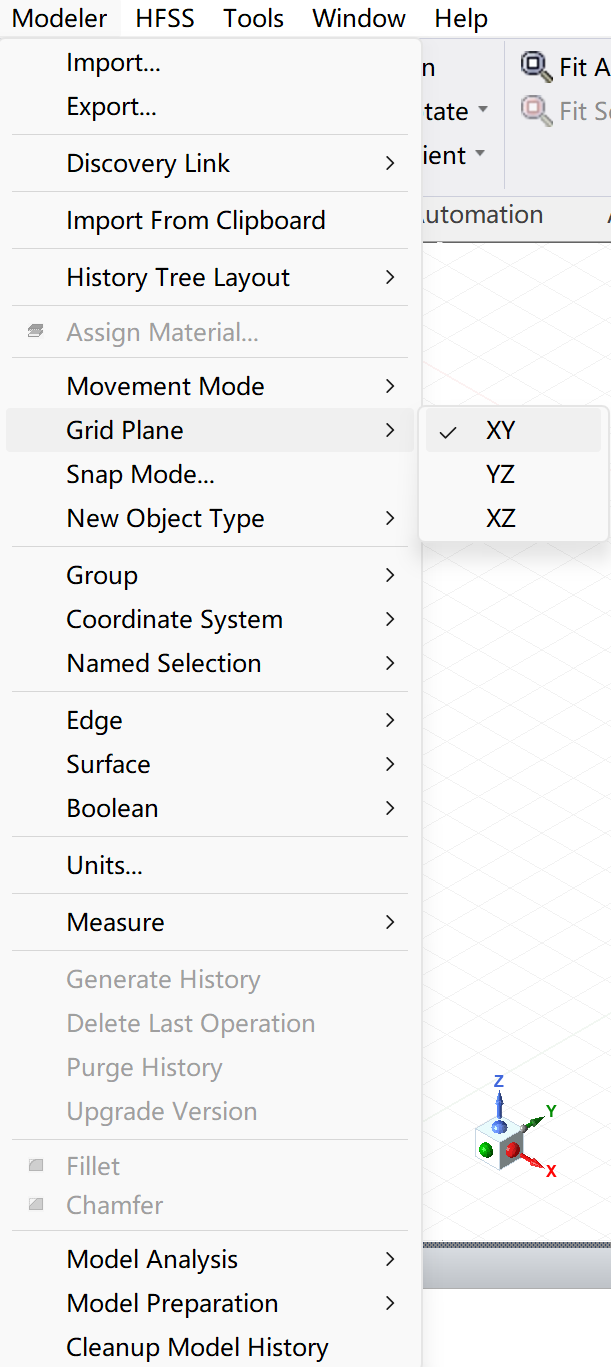
\includegraphics[width=0.3\textwidth]{p8.png}
    \caption{平面设置}
\end{figure}

（2）双击操作历史树中的\keyblue{sheets}下的\keyblue{rectangle1}节点，打开新建矩形面属性对话框，把矩形面的名称设置为\keyblue{Port}；

\begin{figure}[H]
    \centering
    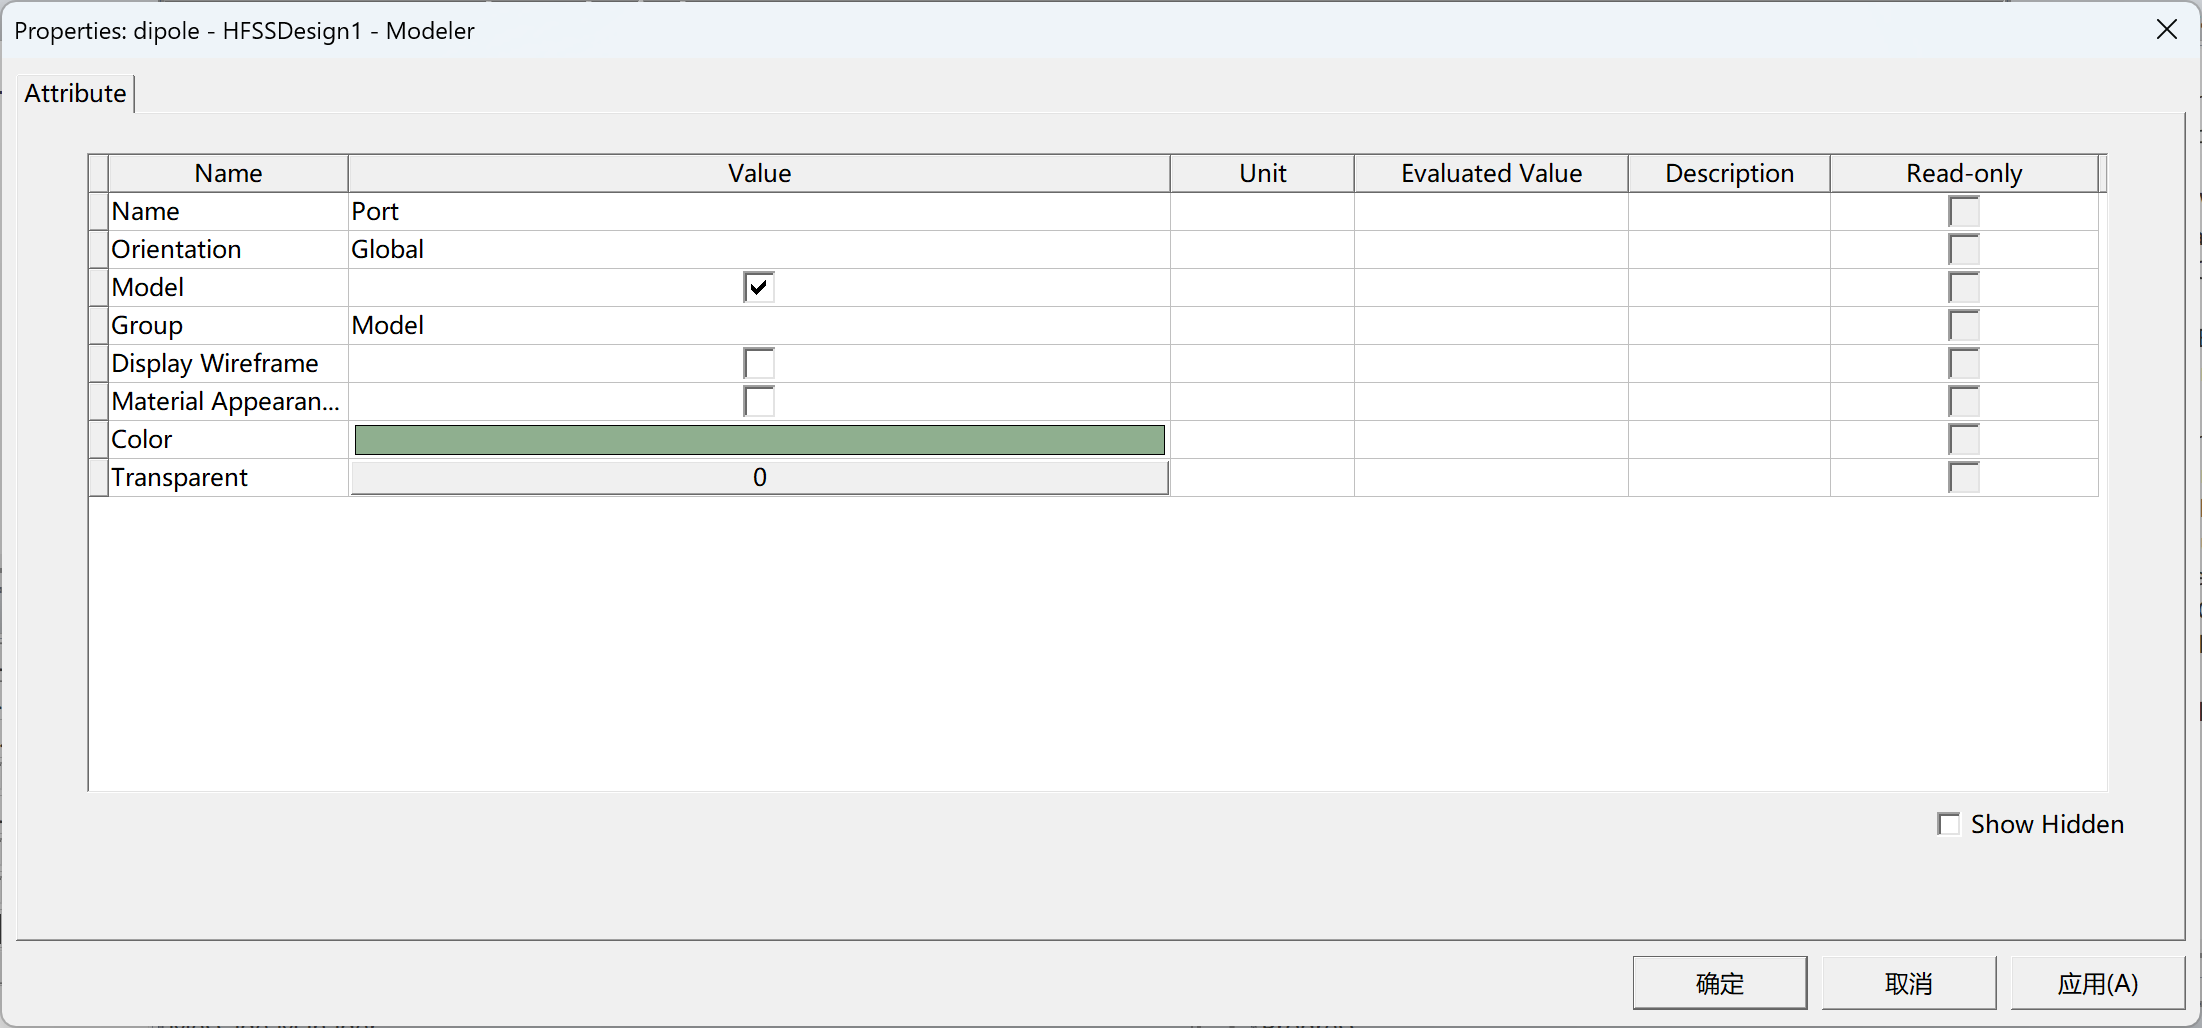
\includegraphics[width=0.8\textwidth]{p10.png}
    \caption{矩形面名称设置}
\end{figure}

（3）双击操作历史树下\keyblue{Port}下的\keyblue{CreateRetangle}节点，在选项卡中设置矩形面的顶点坐标和大小；

\begin{figure}[H]
    \centering
    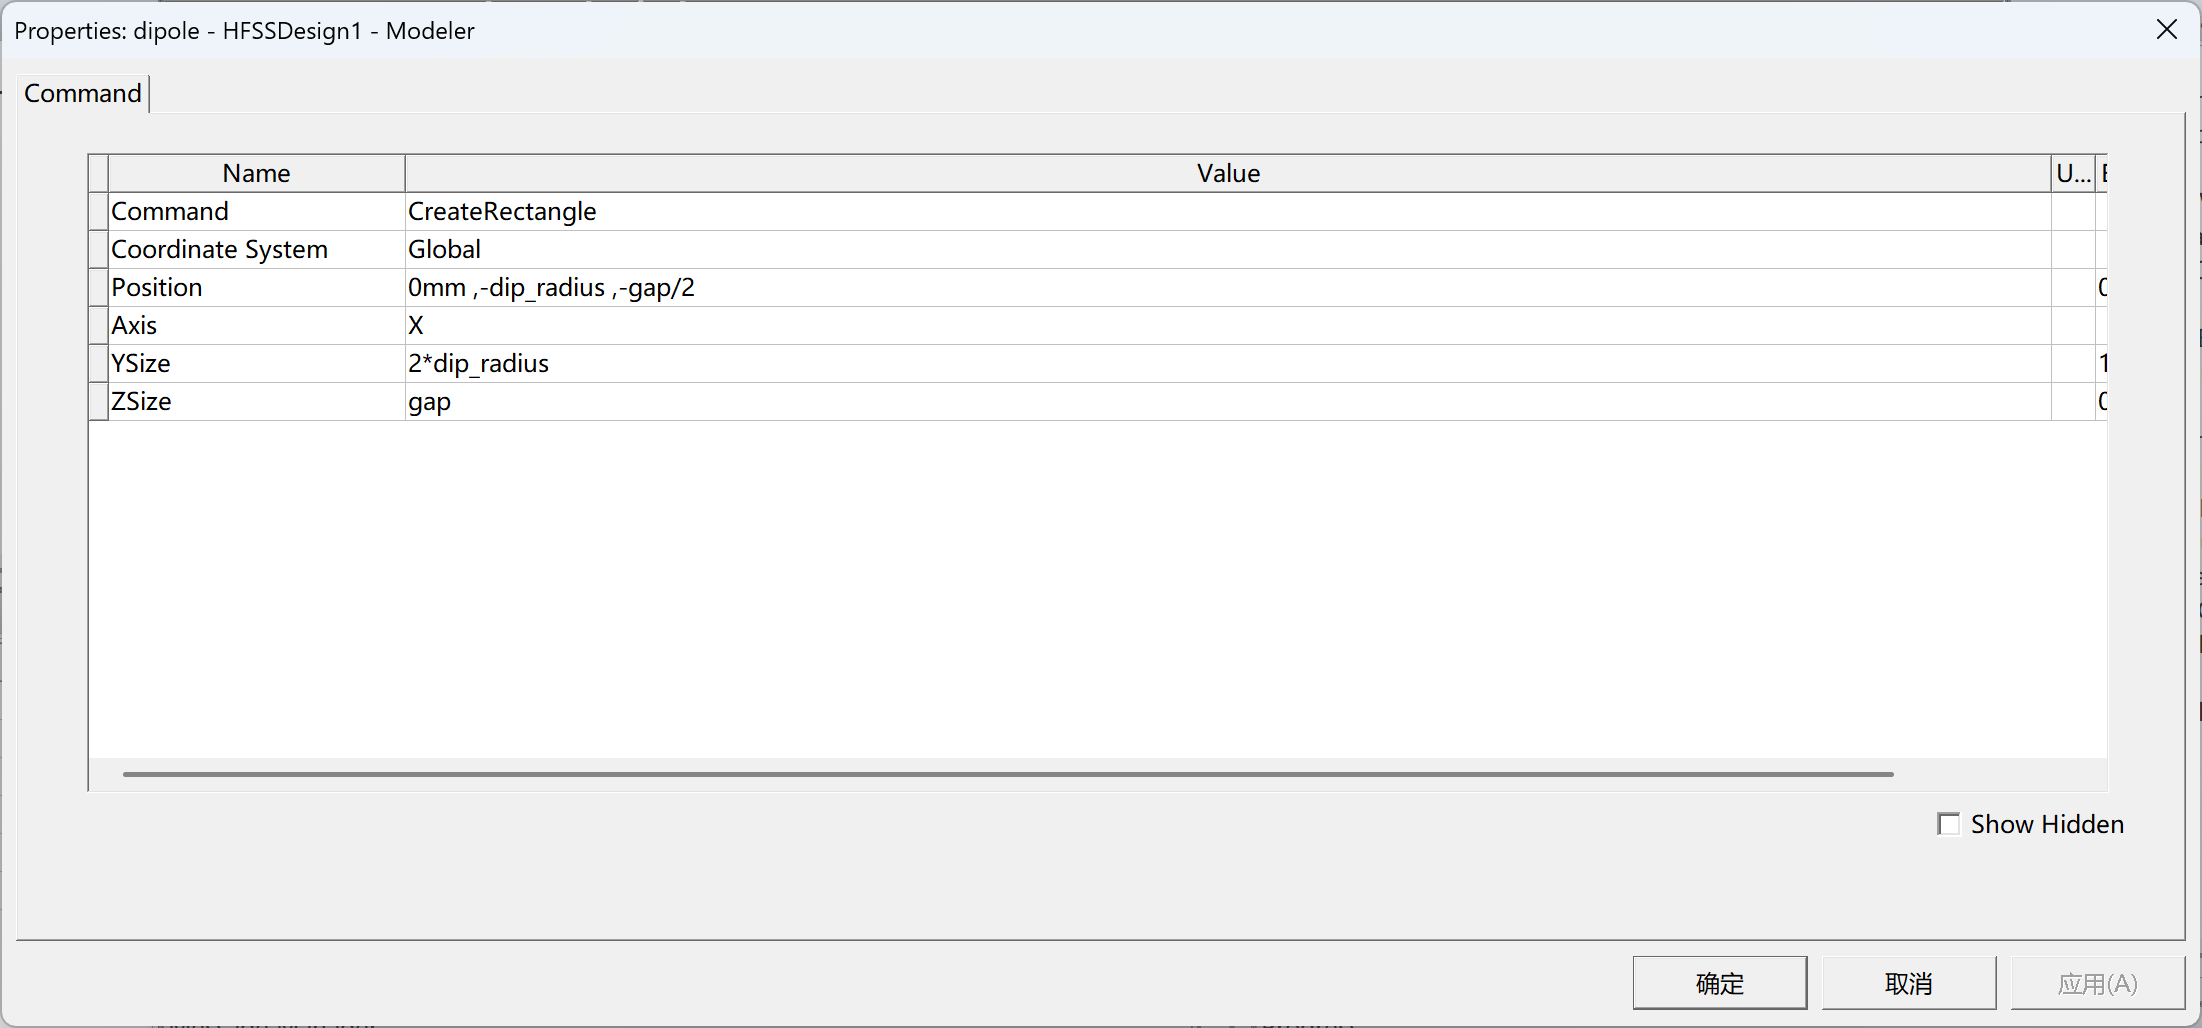
\includegraphics[width=0.8\textwidth]{p11.png}
    \caption{矩形面坐标与大小设置}
\end{figure}

（4）在操作历史树的\keyblue{Sheets}节点下选中\keyblue{Port}，在菜单中选中\keyblue{Assign Excitation}--\keyblue{Port}--\keyblue{Lumped Port}，在打开的集总参数设置对话框中，将\keyblue{Full Port Impedance}设为\keyblue{73.2}$\Omega$，单击下一页；在Modes对话框中单击\keyblue{Integration Line}--\keyblue{None}，从下拉菜单中选择\keyblue{New Line}，在进入的三维模型 窗口中画出一条由下至上的端口积分线，在Port Processing对话框中中选择\keyblue{Do Not Renormalize}，单击完成。

\subsubsection{\heiti\bfseries 设置辐射边界条件}

（1）创建辐射边界的圆柱体：单击工具栏上的 YZ 下拉列表框，从其下拉列表中选择 XY 项，将当前工作平面设置为 XY 平面；

（2）选择菜单栏\keyblue{Draw}–\keyblue{Cylinder}创建圆柱体，将圆柱体名称改为\keyblue{Rad\_air}，设置材质为\keyblue{air}，透明度为\keyblue{0.8}，点击确定，如图：

\begin{figure}[H]
    \centering
    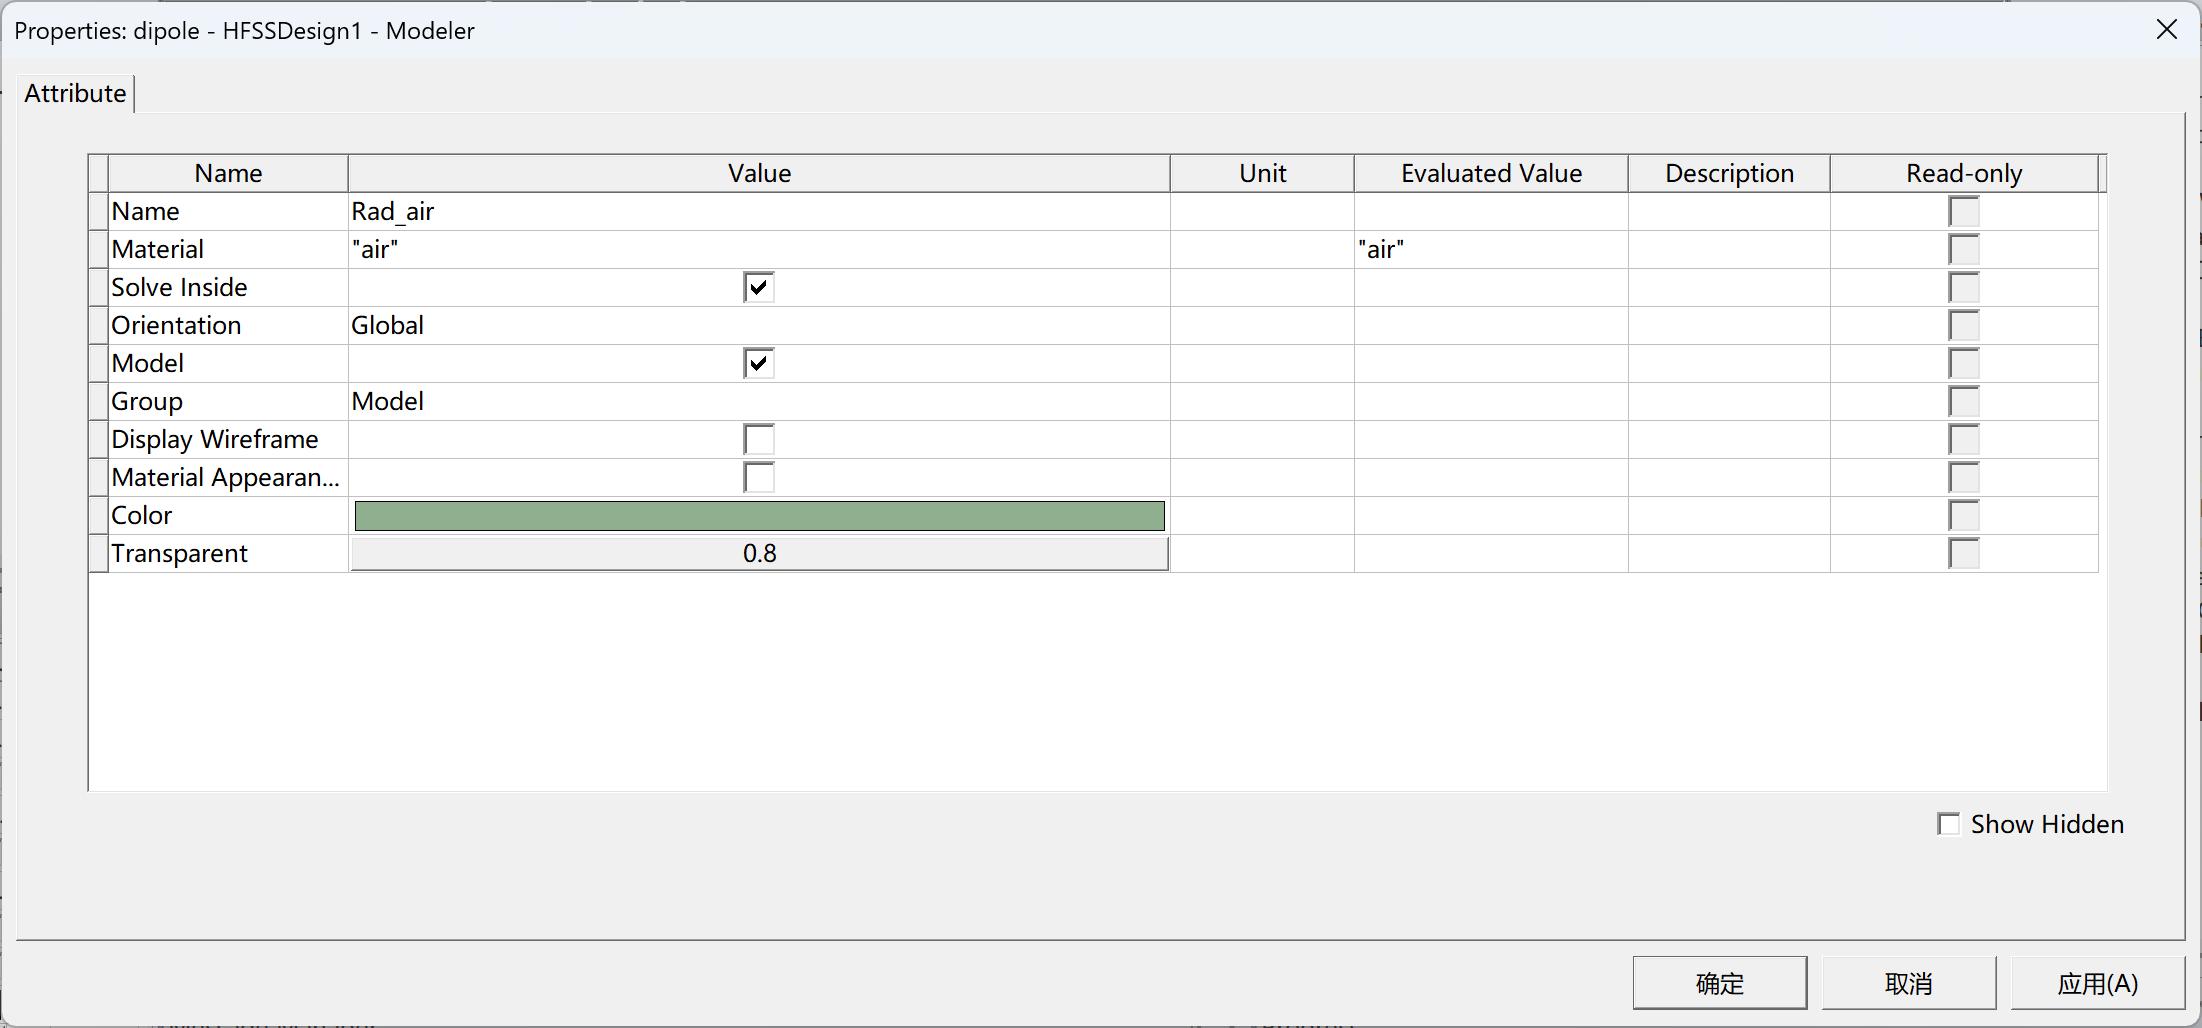
\includegraphics[width=0.8\textwidth]{p15.png}
    \caption{辐射边界圆柱体名称材质设置}
\end{figure}

（3）双击操作历史树中的\keyblue{Rad\_air}下的\keyblue{CreateCylinder}节点，在选项卡中设置尺寸：

\begin{figure}[H]
    \centering
    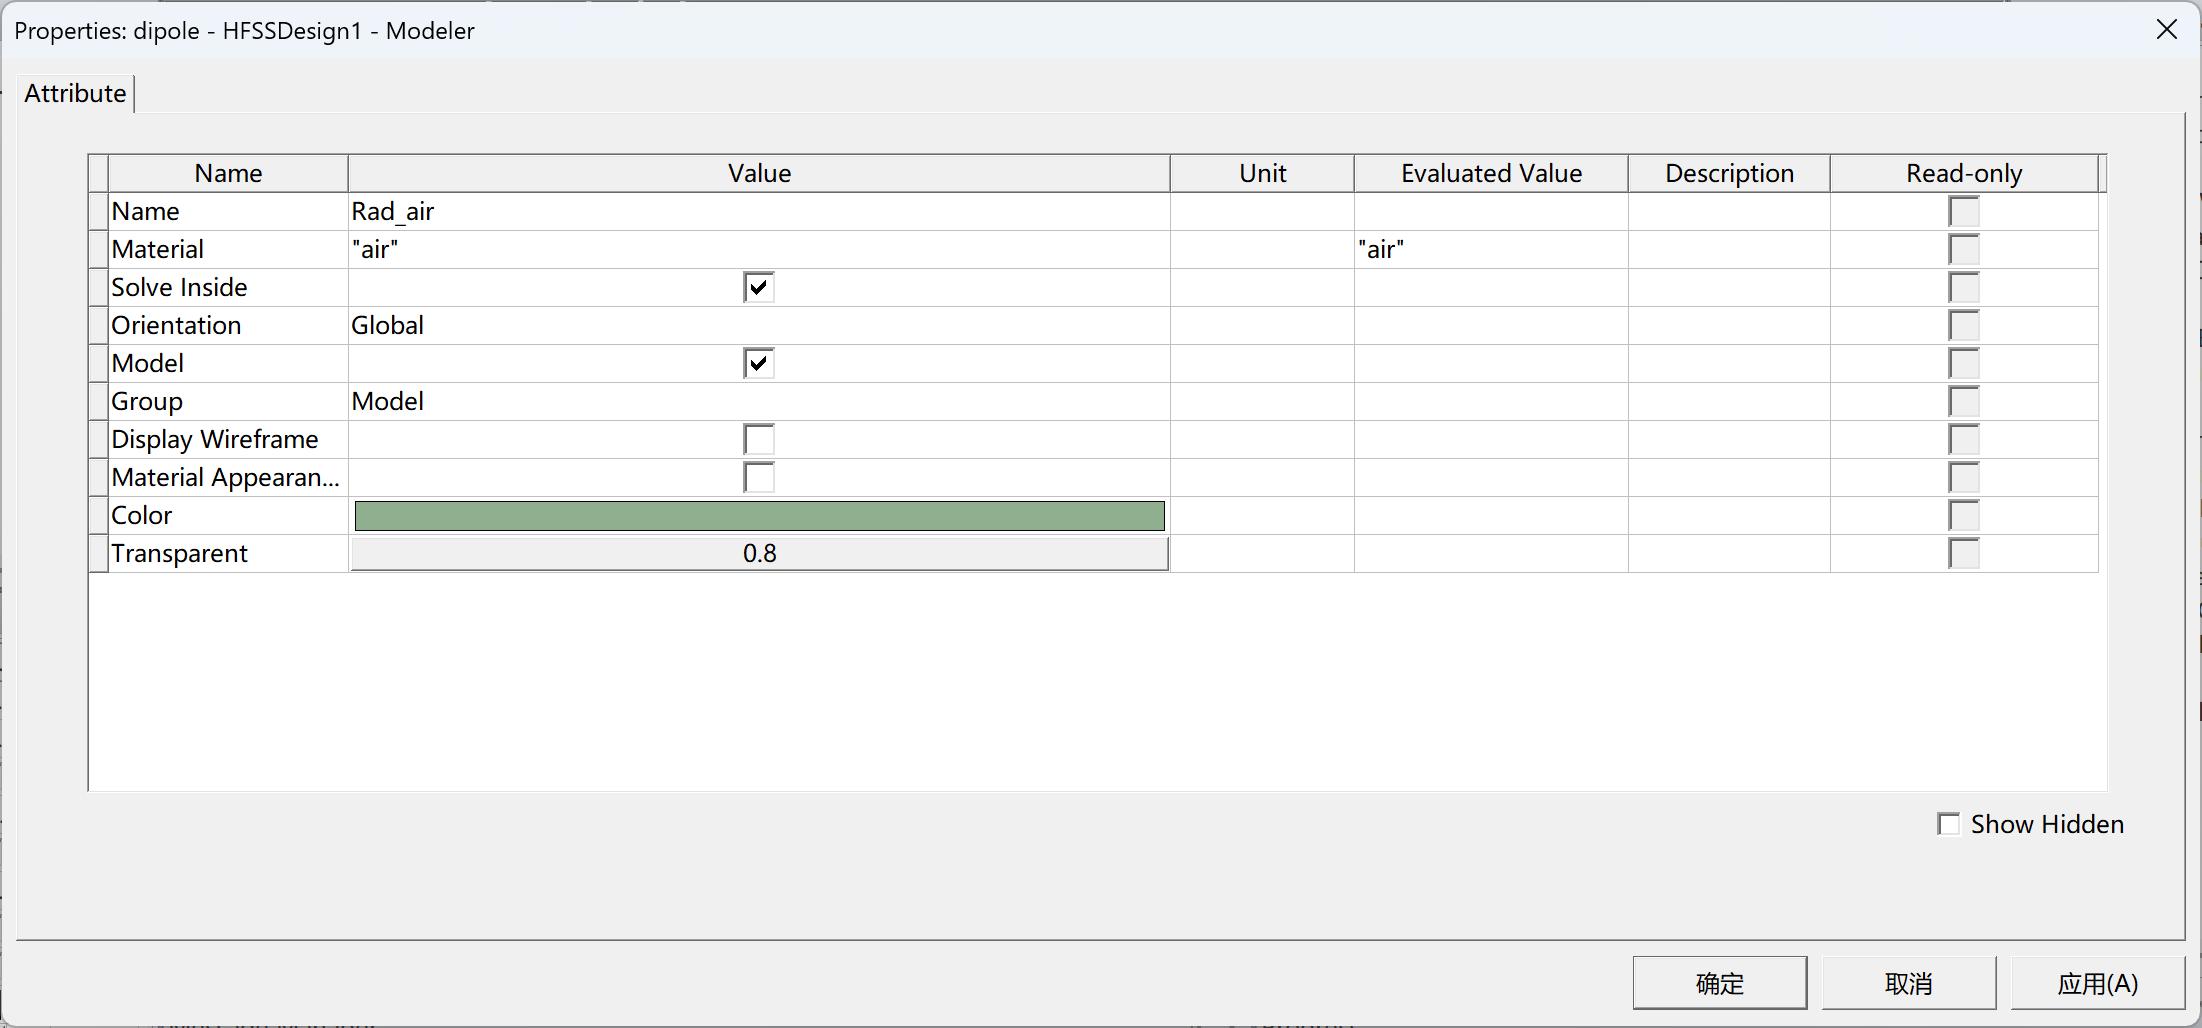
\includegraphics[width=0.8\textwidth]{p15.png}
    \caption{辐射边界圆柱体尺寸设置}
\end{figure}

（4）在操作历史树下单击\keyblue{Rad\_air}节点，在弹出的快捷菜单中选择\keyblue{Assign Boundary}–\keyblue{Radiation}，打开辐射边界条件设置对话框，保留默认设置，从而将\keyblue{Rad\_air}表面设置 为辐射边界条件。

\begin{figure}[H]
    \centering
    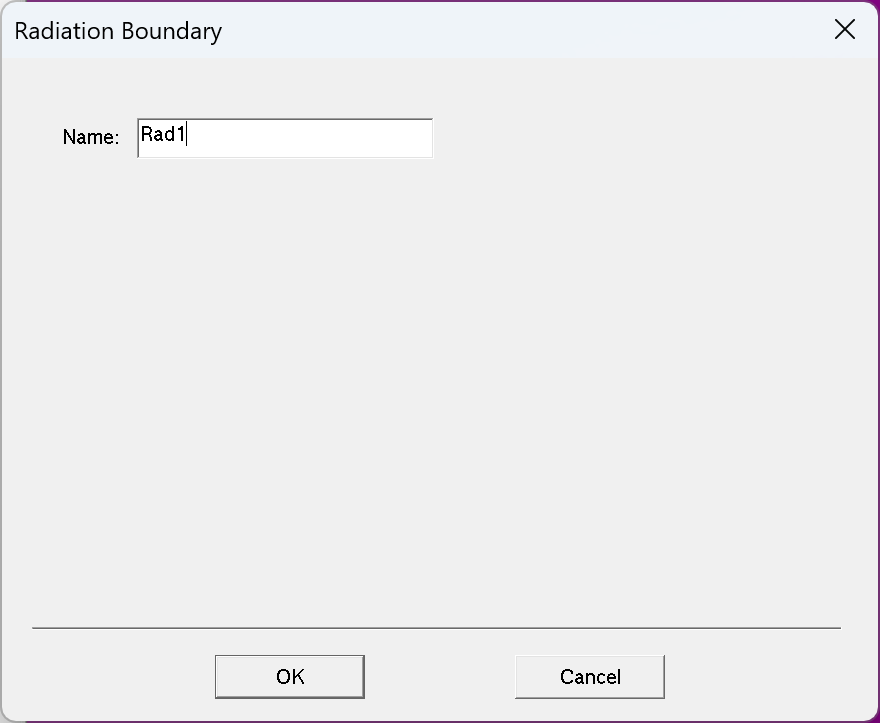
\includegraphics[width=0.8\textwidth]{p17.png}
    \caption{辐射边界圆柱体尺寸设置}
\end{figure}

至此，半波偶极子天线模型建立完毕，完整模型图如下所示：

\begin{figure}[H]
    \centering
    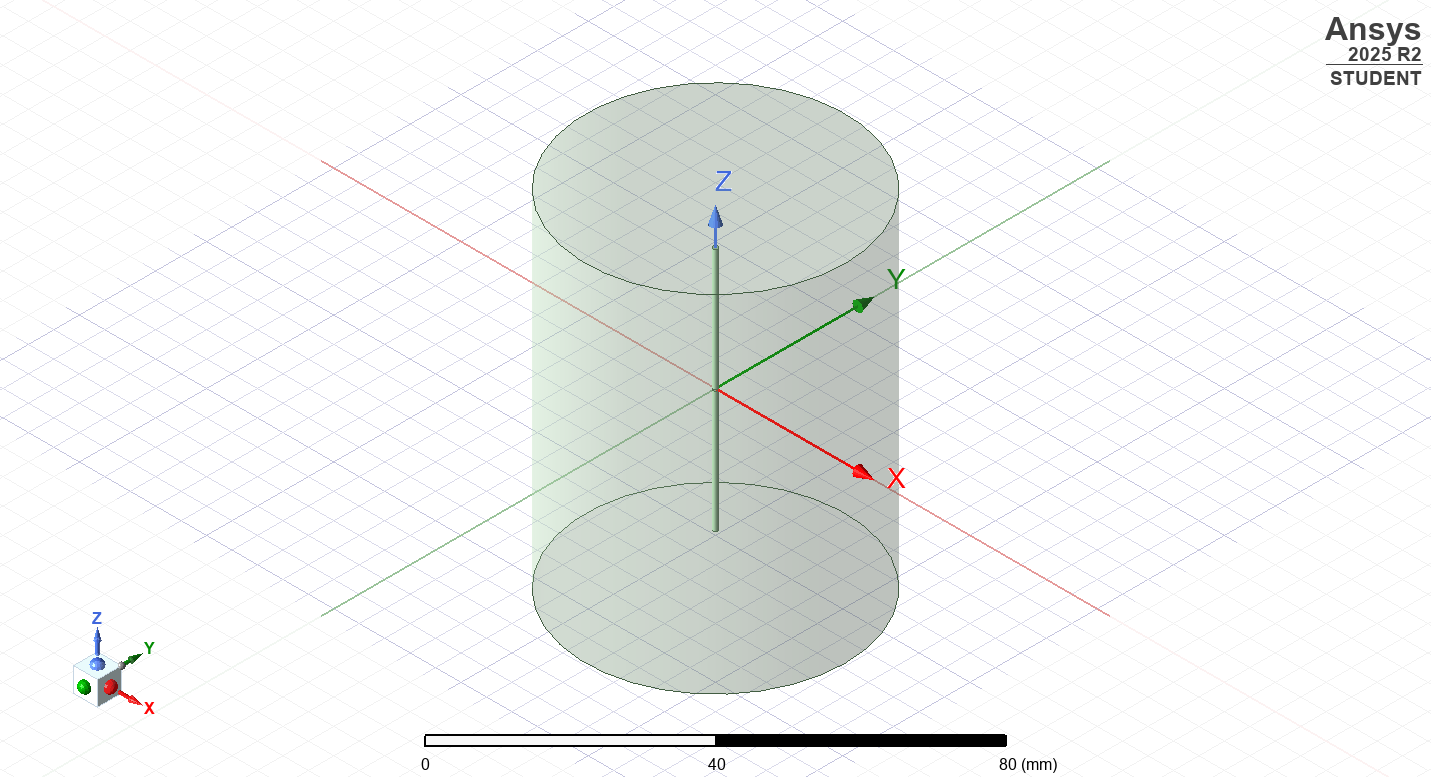
\includegraphics[width=0.8\textwidth]{p18.png}
    \caption{半波偶极子天线完整模型}
\end{figure}

\subsection{\heiti\bfseries 求解设置}
\subsubsection{\heiti\bfseries 求解频率和网格剖分设置}

（1）求解频率和网格剖分设置：右键工程树下的\keyblue{Analysis}，弹出对话框中选中\keyblue{Add Solution Setup}，将求解频率设为 $3GHz$，自适应网格剖分的最大迭代次数设为 \keyblue{20}，收敛误差\keyblue{0.02}，如图所示：

\begin{figure}[H]
    \centering
    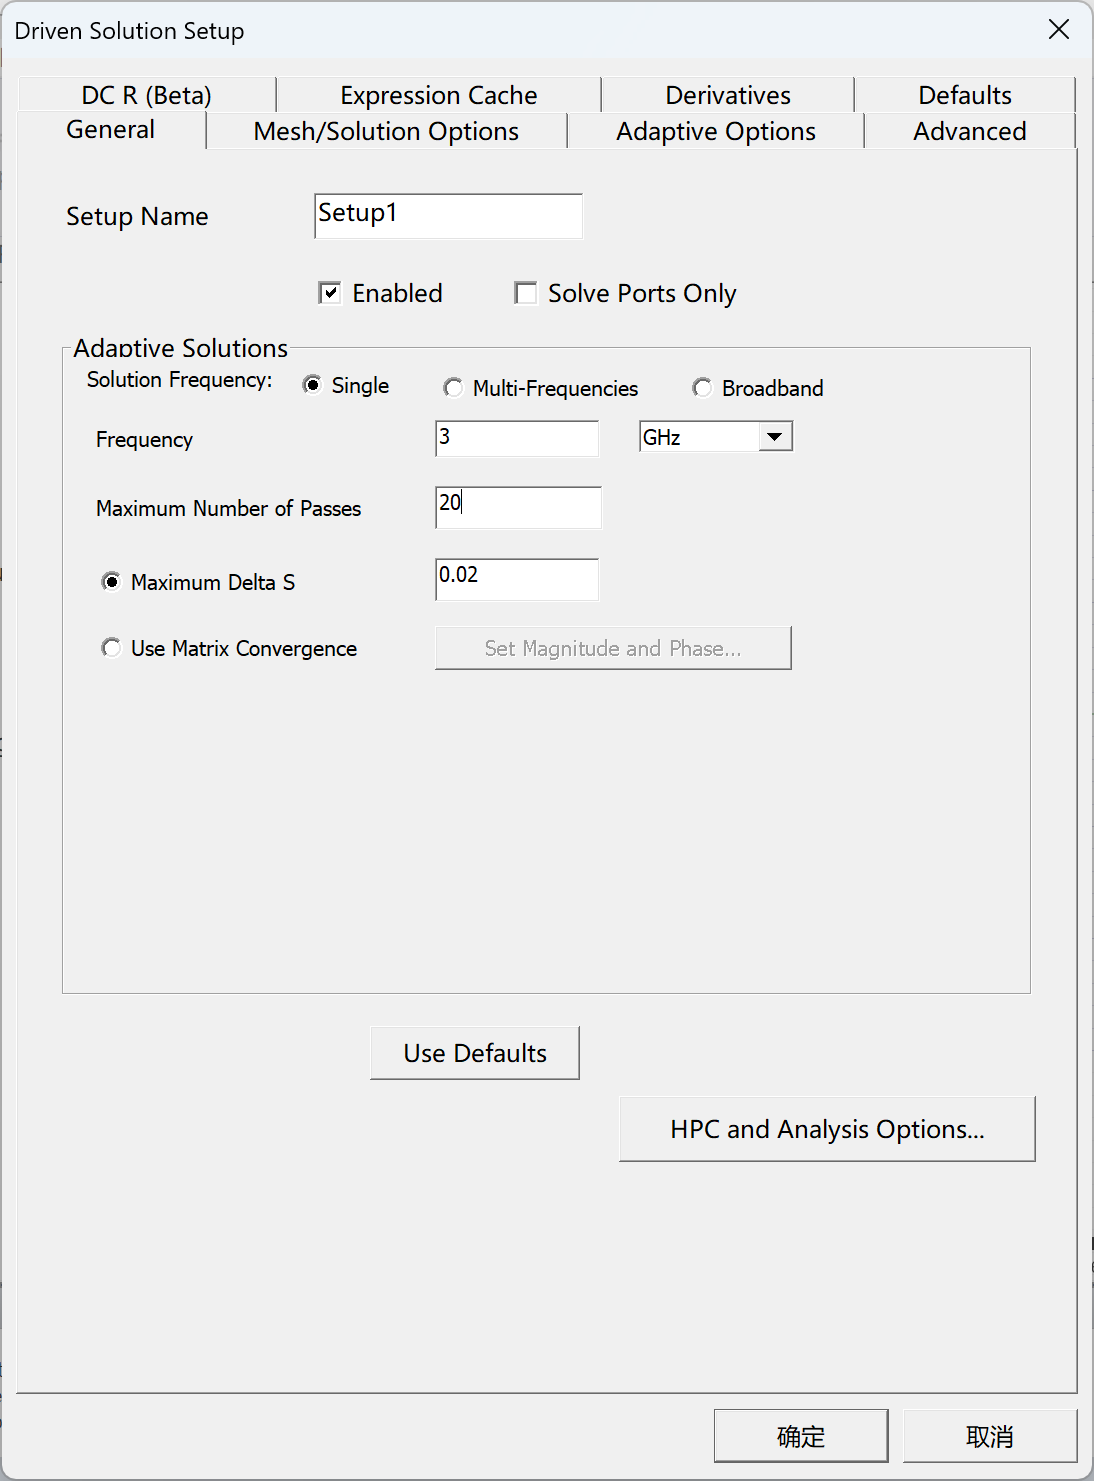
\includegraphics[width=0.8\textwidth]{p20.png}
    \caption{求解频率和网格剖分设置}
\end{figure}

\subsubsection{\heiti\bfseries 扫频设置}

（2）扫频设置：展开工程树下的\keyblue{Analysis}节点，右键单击求解设置项\keyblue{Setup1}，在弹出的对话框中选择\keyblue{Add Frequency Sweep}，扫频类型为快速扫频，扫频范围 $2.5GHz - 3.5GHz$，点数为\keyblue{1000}：

\begin{figure}[H]
    \centering
    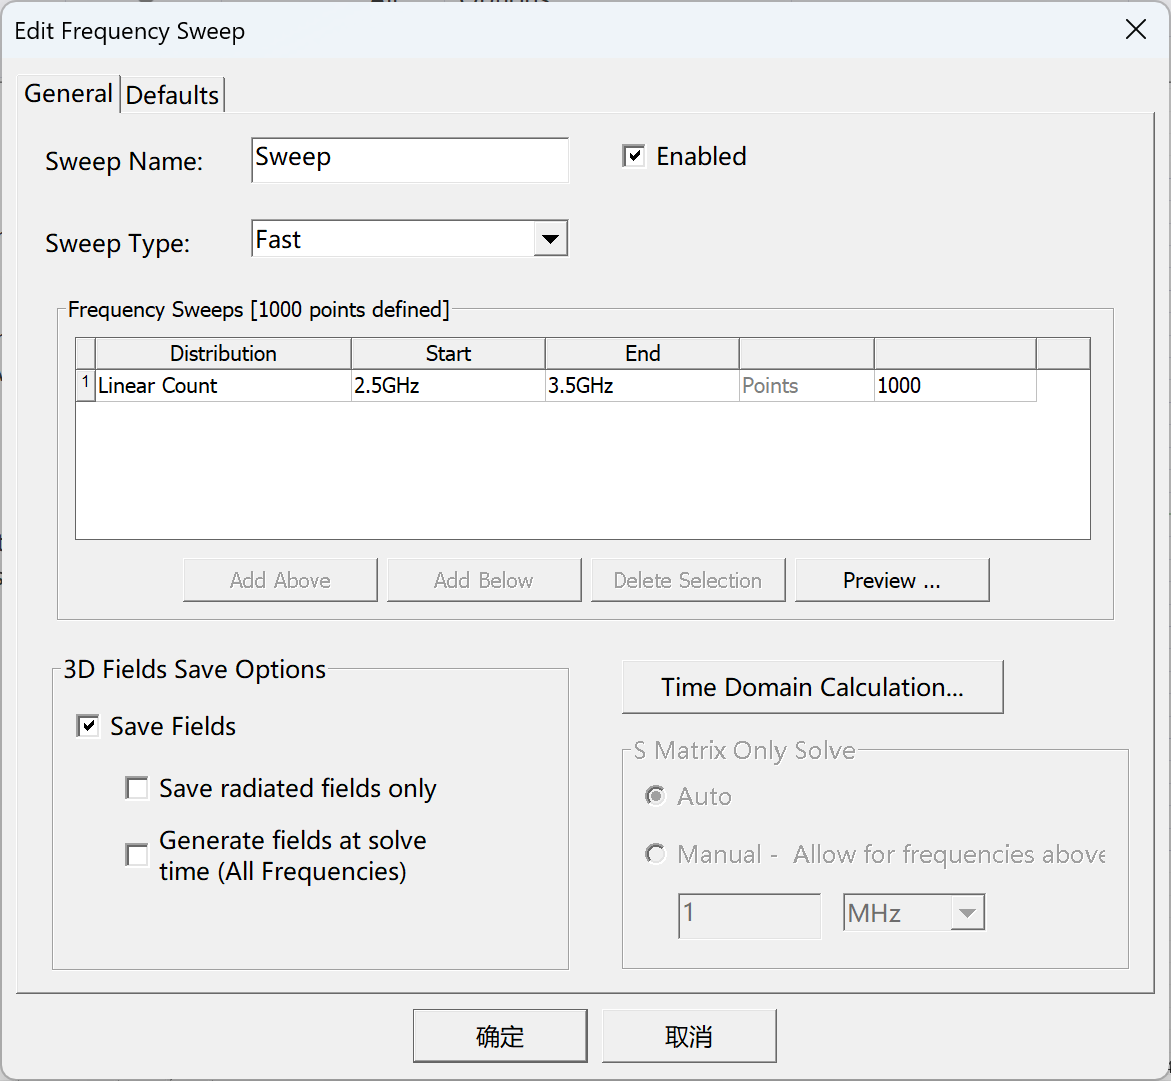
\includegraphics[width=0.8\textwidth]{p21.png}
    \caption{扫频设置}
\end{figure}

\subsection{\heiti\bfseries 设计检查和运行仿真运算}

（1）选择主菜单中\keyblue{HFSS}–\keyblue{Validation Check}，得到如下对话框，表明设计正确：

\begin{figure}[H]
    \centering
    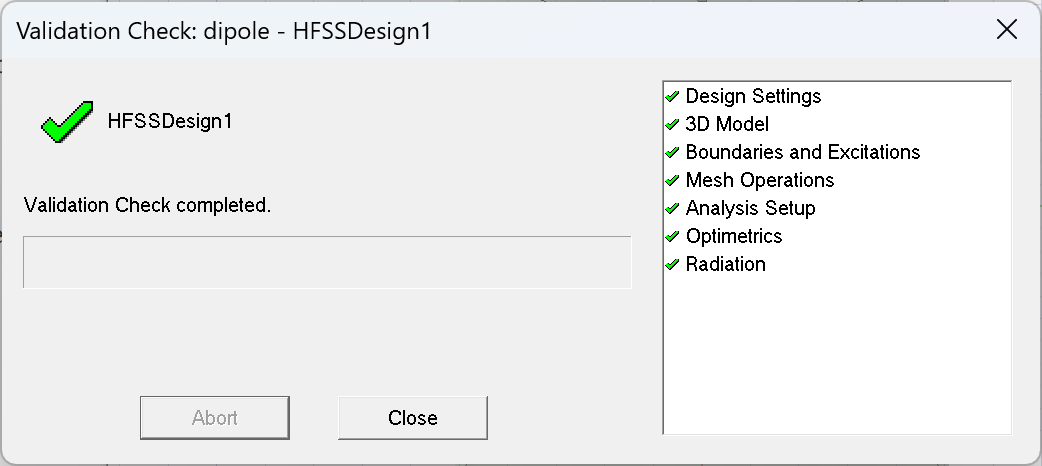
\includegraphics[width=0.8\textwidth]{p22.png}
    \caption{设计验证}
\end{figure}

（2）右键单击工程树下的\keyblue{Analysis}—\keyblue{Setup1}，在弹出菜单中选择\keyblue{Analyze}，运行分析。

\section{\heiti\bfseries HFSS天线数据后处理}

仿真分析完成后，在数据后处理部分能够给出天线的各项性能参数的仿真分析结果，如回波损耗、驻波比、Smith圆图、输入阻抗和方向图等。

\subsection{\heiti\bfseries 回波损耗}

右键单击工程树下的\keyblue{Results}节点，在弹出的菜单中选择\keyblue{Create Model Solution Data Report}—\keyblue{Rectangle Plot}命令，打开报告设置对话框，如图所示：

\begin{figure}[H]
    \centering
    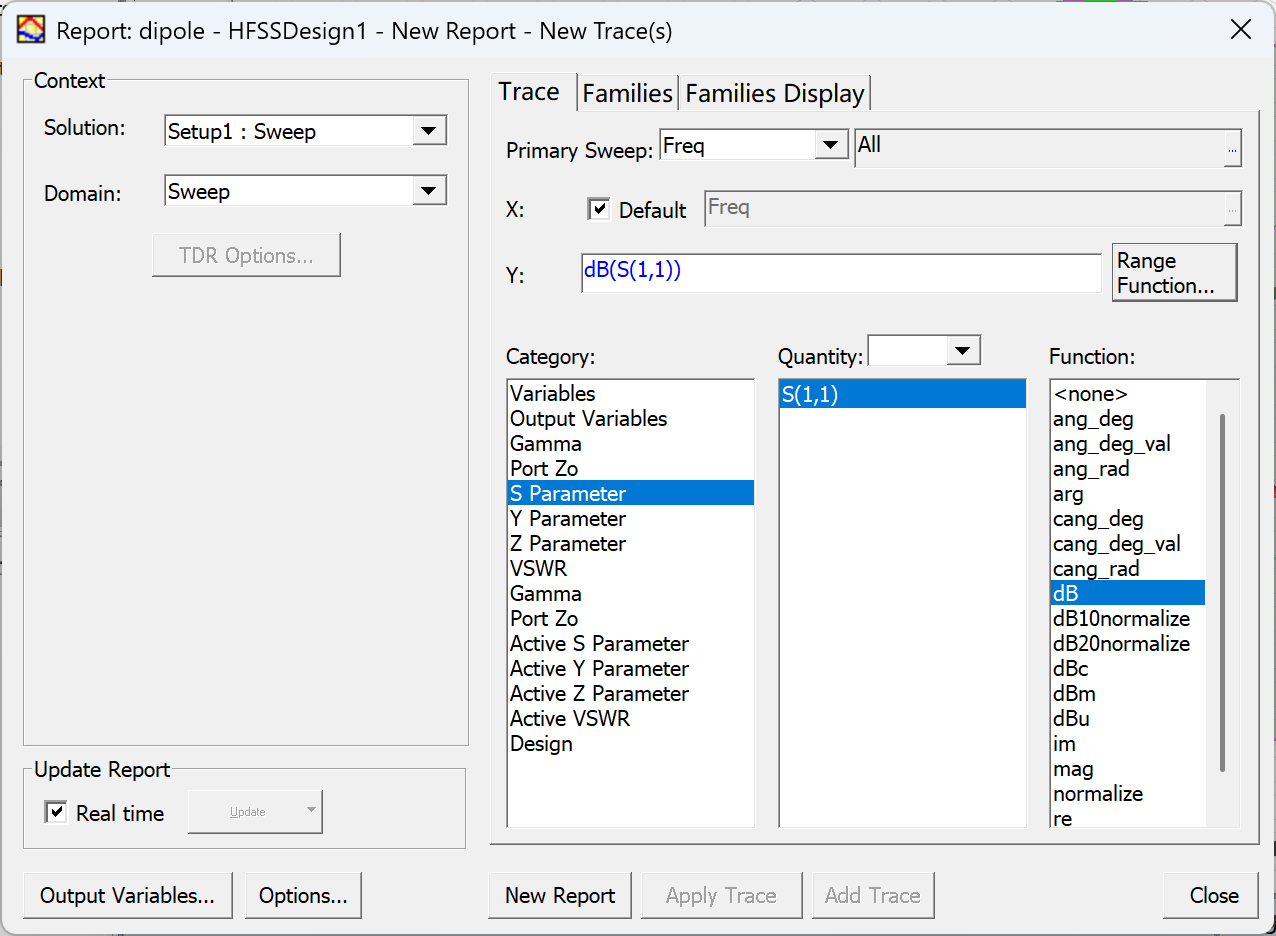
\includegraphics[width=0.8\textwidth]{p23.png}
    \caption{回波损耗报告设置}
\end{figure}

单击\keyblue{New Report}按钮，此时可以生成 $2.5GHz - 3.5GHz$ 频段内回波损耗$S_{11}$分析结果：

\begin{figure}[H]
    \centering
    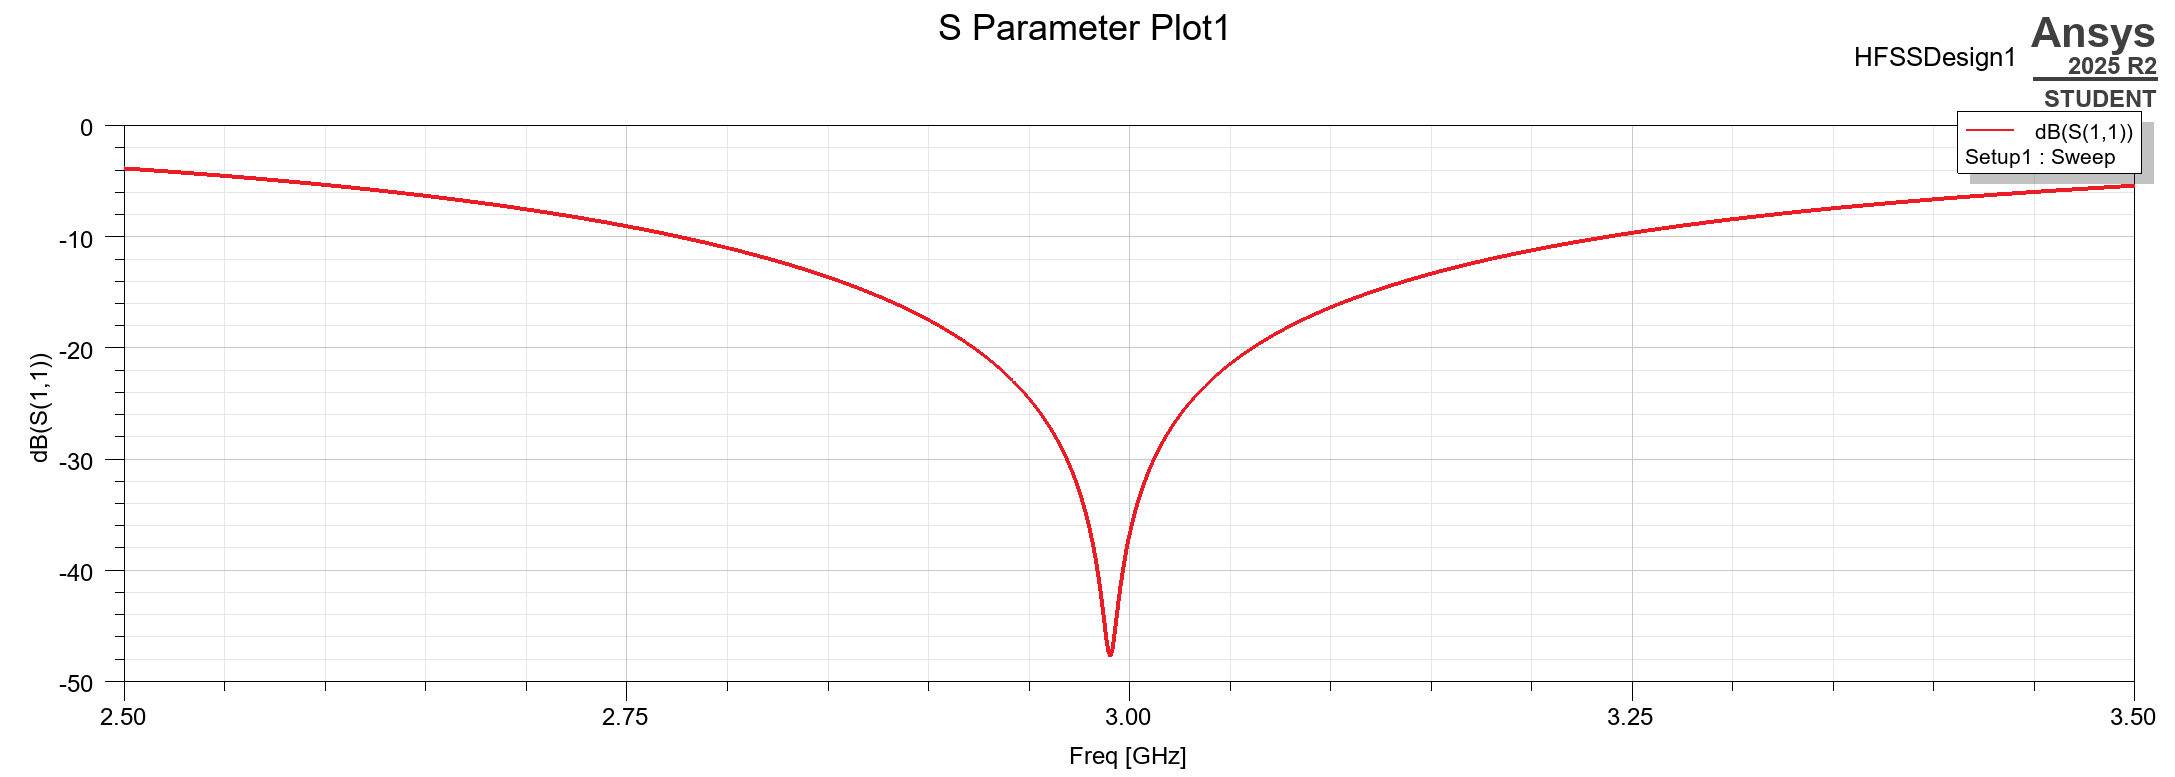
\includegraphics[width=0.8\textwidth]{p24.png}
    \caption{回波损耗$S_{11}$分析结果}
\end{figure}

【实验结果】:由图可知，半波偶极子天线在 $2.78GHz - 3.25GHz$ 之间的回波损耗 $S_{11}$ 小于 $-10dB$，此时天线处于较理想匹配状态，能够将大部分能量辐射出去，有优良的辐射特性；当工作频率为 $3.00GHz$ 左右时，天线的回波损耗最小，约为 $-47dB$，计算可得天线 $S_{11} < 10dB$ 相对带宽：
\begin{equation}
BW = \frac{3.25 - 2.78}{3} = 15.6\%
\end{equation}
结果表明，该天线在中心频率附近具有良好的阻抗匹配特性。

\subsection{\heiti\bfseries 电压驻波比}

右键单击工程树下的\keyblue{Results}节点，在菜单中选择\keyblue{Create Model Solution Data Report}—\keyblue{Rectangle Plot}命令，打开报告设置对话框，按下图设置：

\begin{figure}[H]
    \centering
    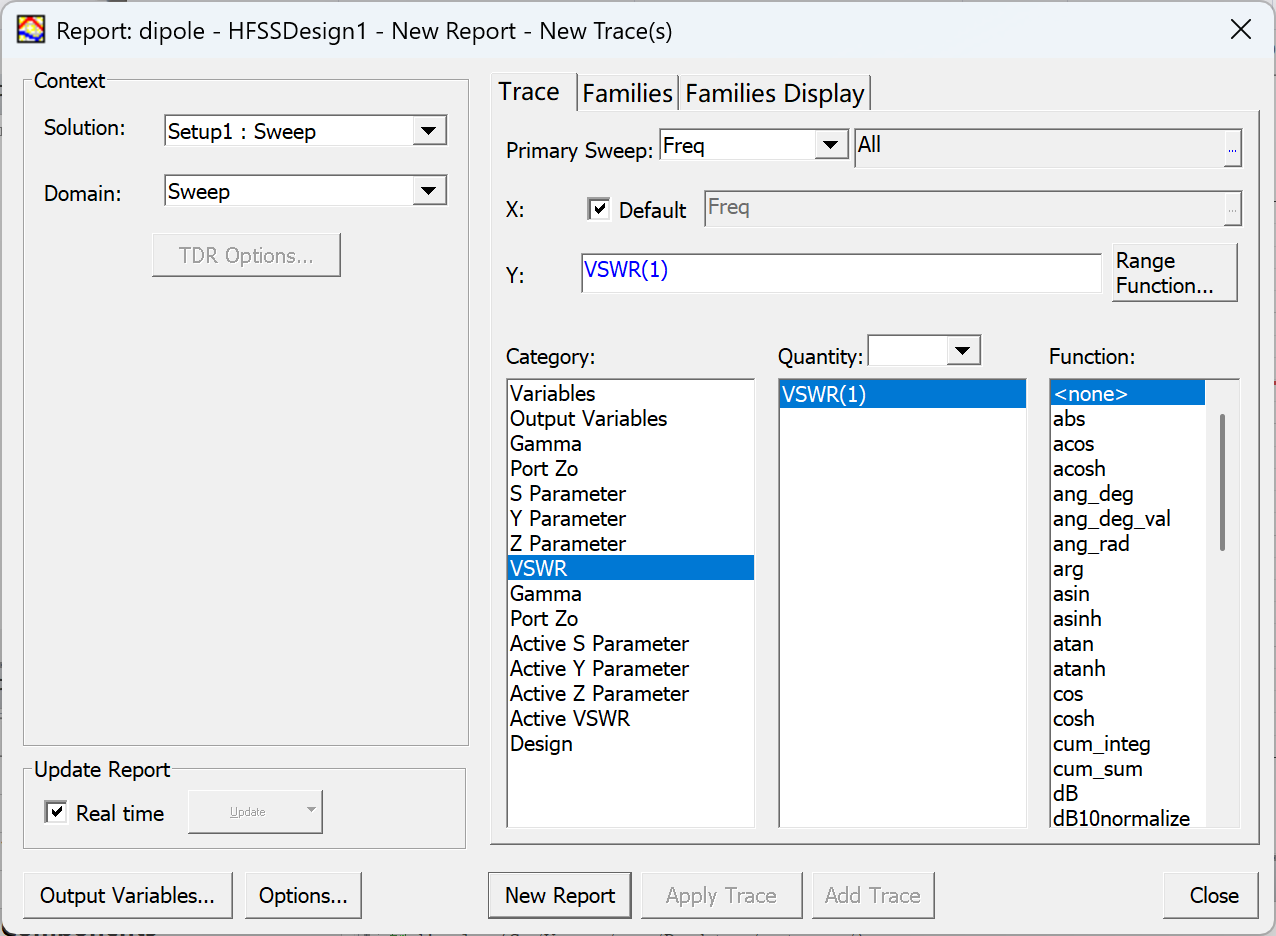
\includegraphics[width=0.8\textwidth]{p25.png}
    \caption{驻波比报告设置}
\end{figure}

单击\keyblue{New Report}，得到天线的驻波比分析结果：

\begin{figure}[H]
    \centering
    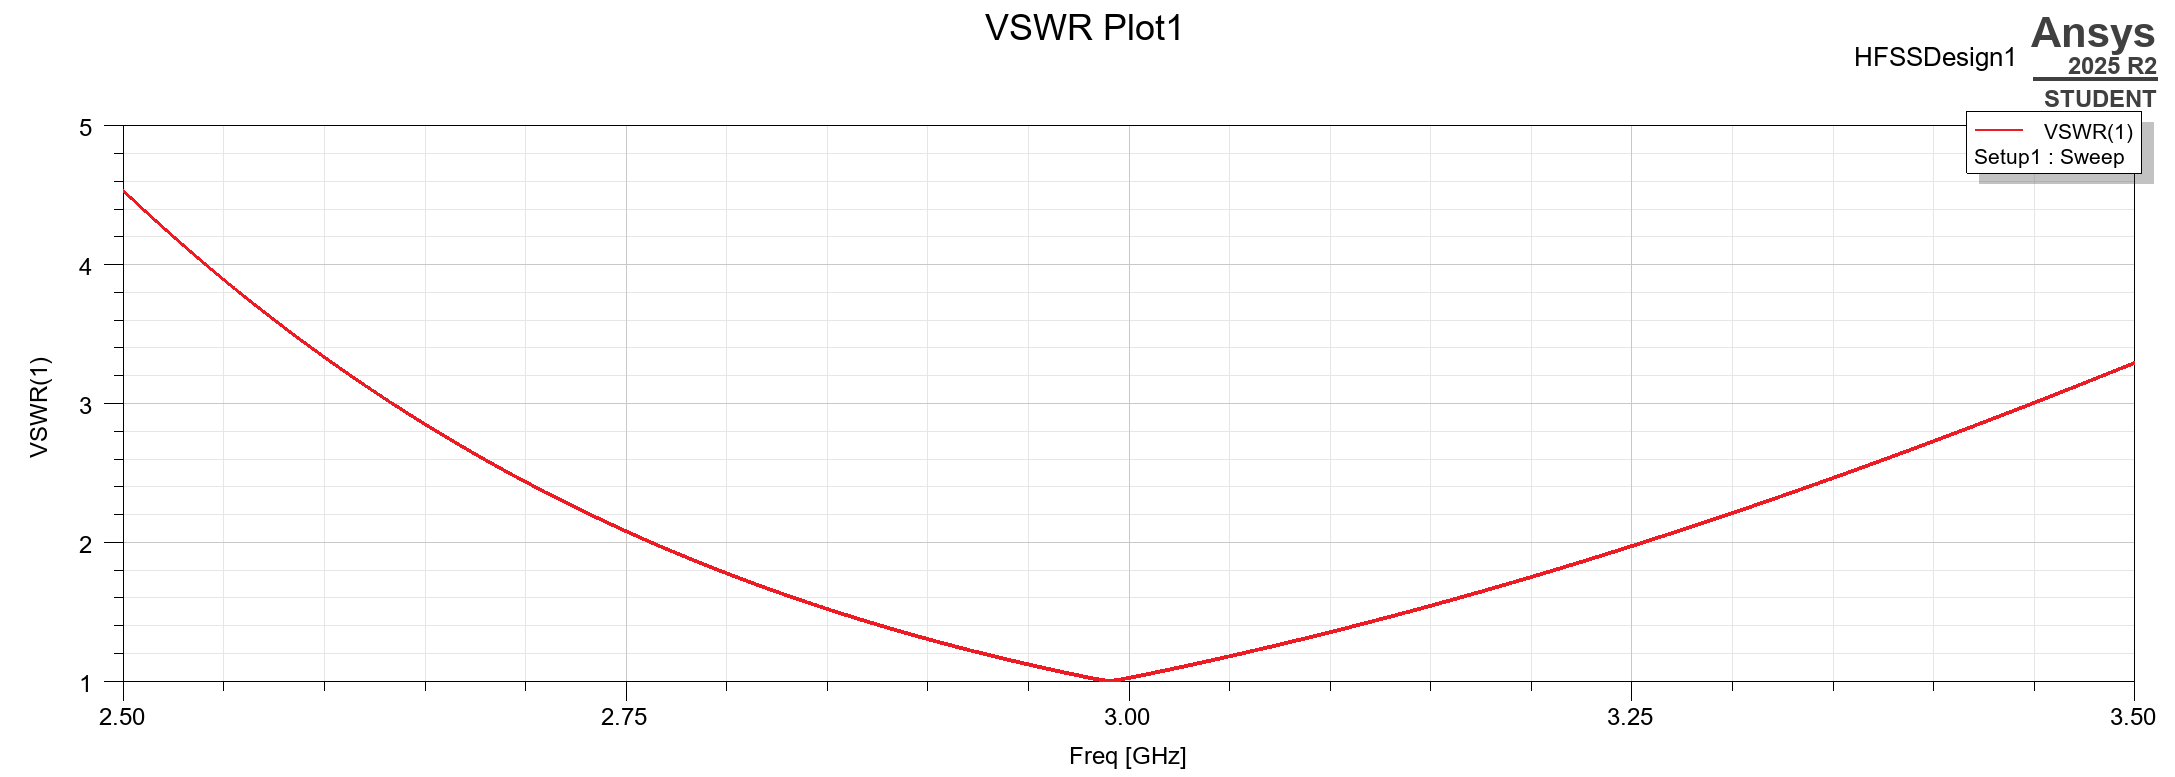
\includegraphics[width=0.8\textwidth]{p26.png}
    \caption{驻波比分析结果}
\end{figure}

【实验结果】:由图可知，天线的电压驻波比 (VSWR) 与回波损耗结果对应良好。在中心频率 3.00 GHz 处，VSWR 值接近理想值 1.0，表明此时天线与馈电端口的阻抗匹配最佳，能量反射最小。
此时传输特性接近行波状态，性能理想。

\subsection{\heiti\bfseries Smith圆图}

右键单击工程树下的Results节点，在弹出的菜单中选择\keyblue{Create Model Solution Data Report}—\keyblue{Smith Chart}，打开如下对话框，进行设置：

\begin{figure}[H]
    \centering
    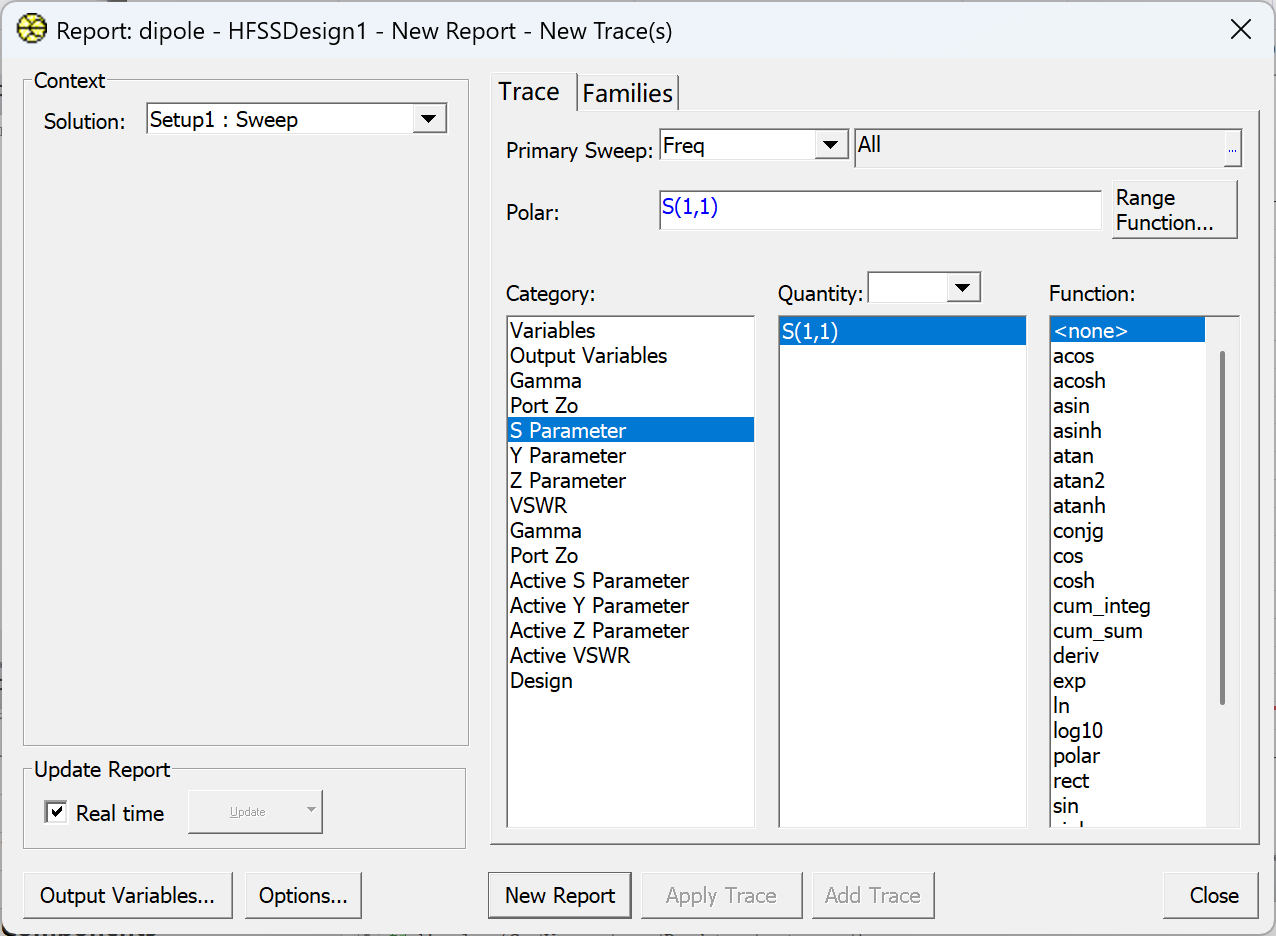
\includegraphics[width=0.8\textwidth]{p27.png}
    \caption{Smith圆图报告设置}
\end{figure}

单击\keyblue{New Report}，得到天线的Smith圆图分析结果：

\begin{figure}[H]
    \centering
    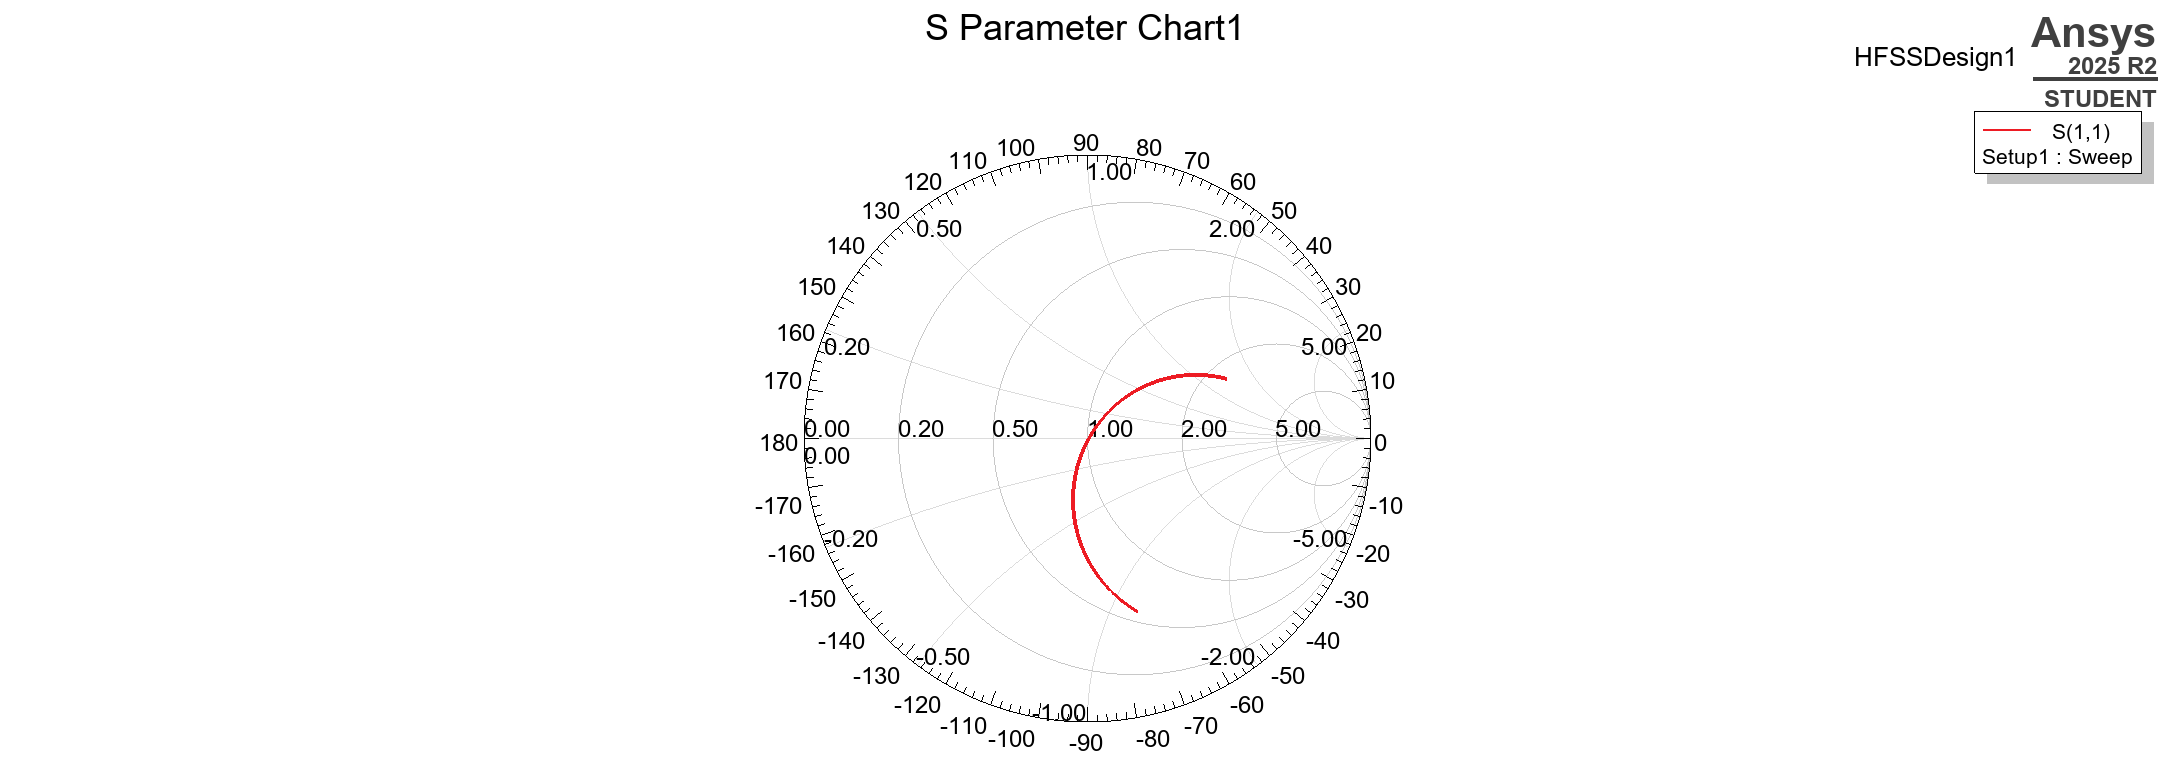
\includegraphics[width=0.8\textwidth]{p28.png}
    \caption{Smith圆图分析结果}
\end{figure}

【实验结果】:由图可知，在中心频率 3.00 GHz 附近，曲线经过圆图中心点 (归一化阻抗 Z=1)，表明阻抗匹配状态理想。
当频率低于 3.00 GHz 时，轨迹点位于圆图下半部分，天线输入阻抗呈现容性。 
当频率高于 3.00 GHz 时，轨迹点位于圆图上半部分，天线输入阻抗呈现感性。 
该阻抗变化规律与理论预期完全一致。
\subsection{\heiti\bfseries 输入阻抗}

右键单击工程树下的Results节点，在弹出的菜单中选择\keyblue{Create Model Solution Data Report}—\keyblue{Rectangle Plot}命令，打开报告设置对话框，如下设置：

\begin{figure}[H]
    \centering
    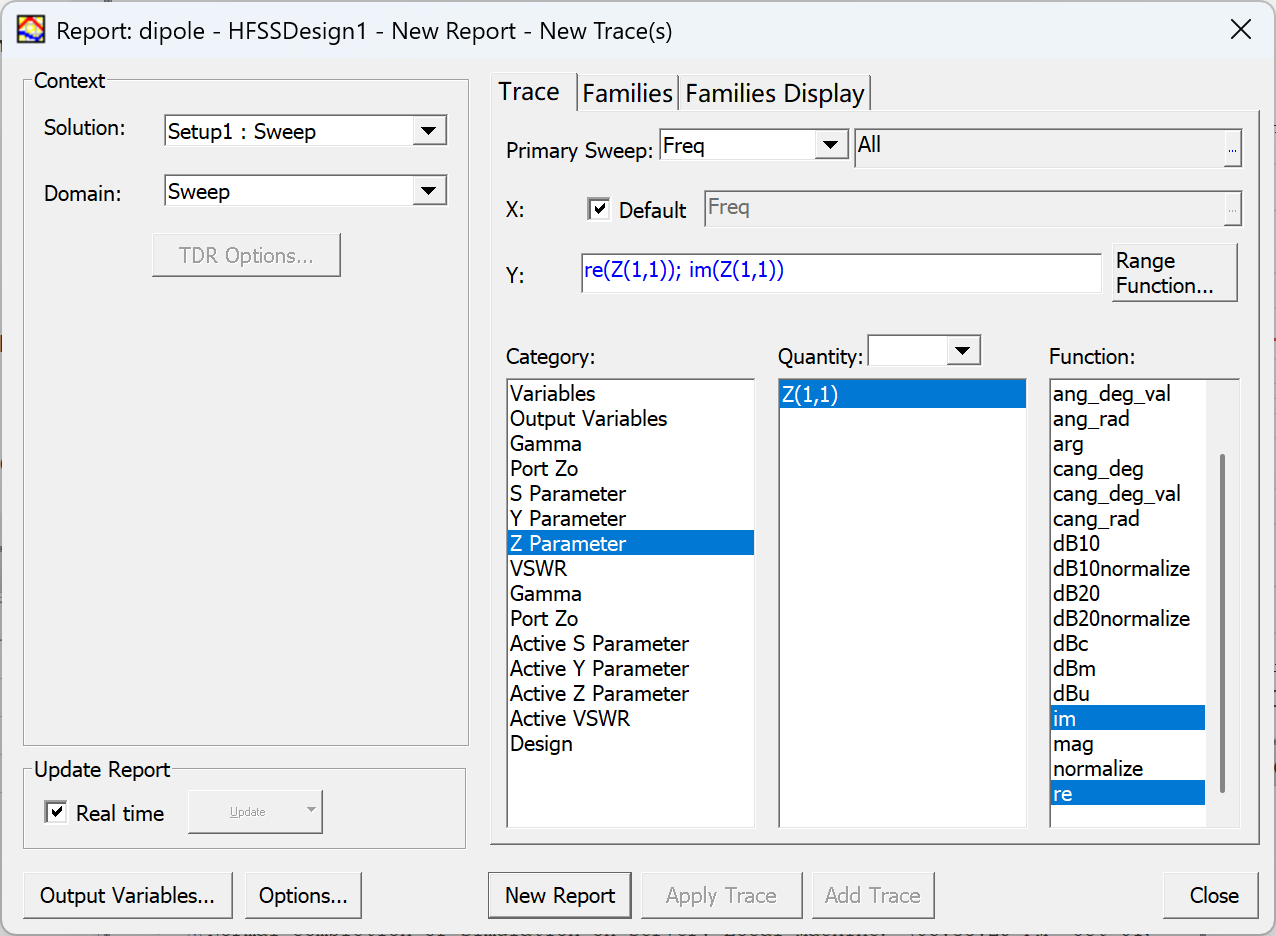
\includegraphics[width=0.8\textwidth]{p29.png}
    \caption{输入阻抗报告设置}
\end{figure}

单击\keyblue{New Report}，得到天线的输入阻抗结果报告：

\begin{figure}[H]
    \centering
    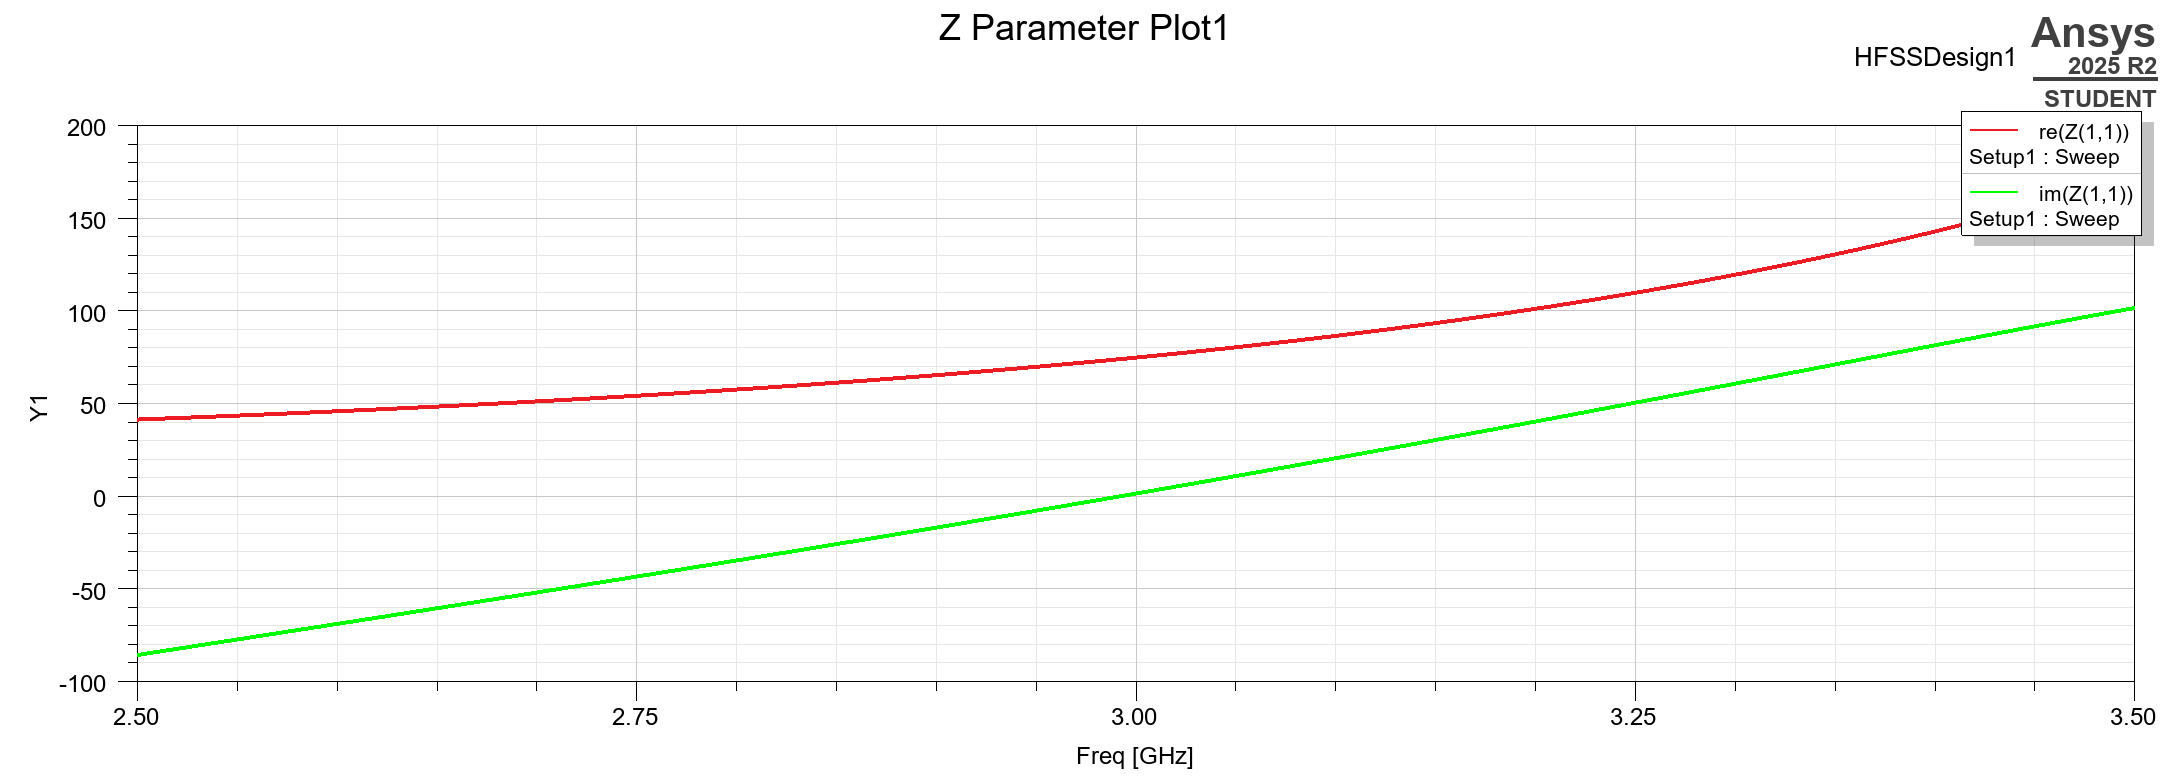
\includegraphics[width=0.8\textwidth]{p30.png}
    \caption{输入阻抗分析结果}
\end{figure}

【实验结果】:由图可知，当工作频率为 $3GHz$ 左右时，天线的阻抗实部接近 $73.2\Omega$，虚部近似为零；当频率小于 $3GHz$ 时，天线电抗为负，呈容性；当频率大于 $3GHz$ 时，天线电抗为正，呈感性。仿真结果与理论分析相一致。

\subsection{\heiti\bfseries 方向图}

（1）定义辐射表面：右键单击工程树下的\keyblue{Radiation}节点，在弹出的快捷菜单中选择\keyblue{Insert Far Field Setup}—\keyblue{Infinite Sphere}，打开\keyblue{Far Radiation Sphere Setup}，依次完成以下设置；

 \begin{figure}[H]
        \centering
        \subcaptionbox{E-plane设置}[0.33\textwidth][c]{
            \centering
            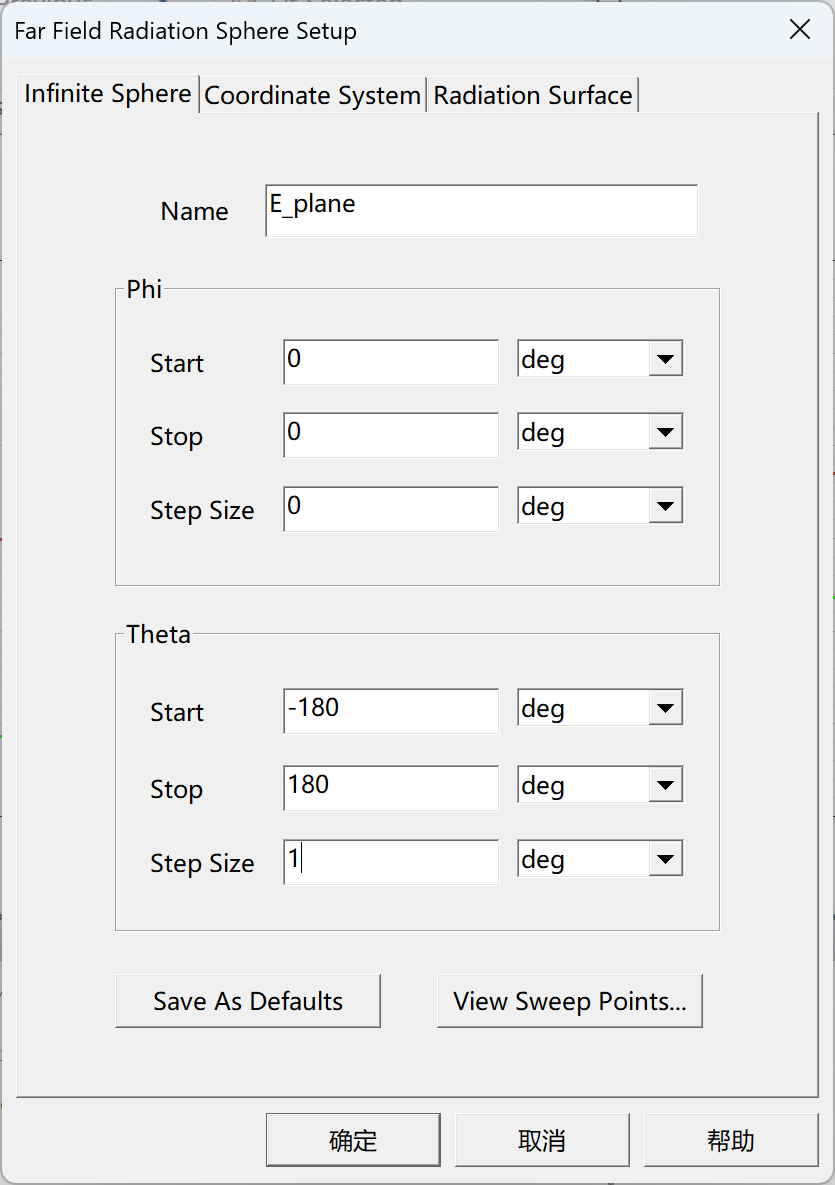
\includegraphics[width=0.32\textwidth]{p31.png}
             
        }%
            \subcaptionbox{H-plane设置}[0.33\textwidth][c]{
            \centering
            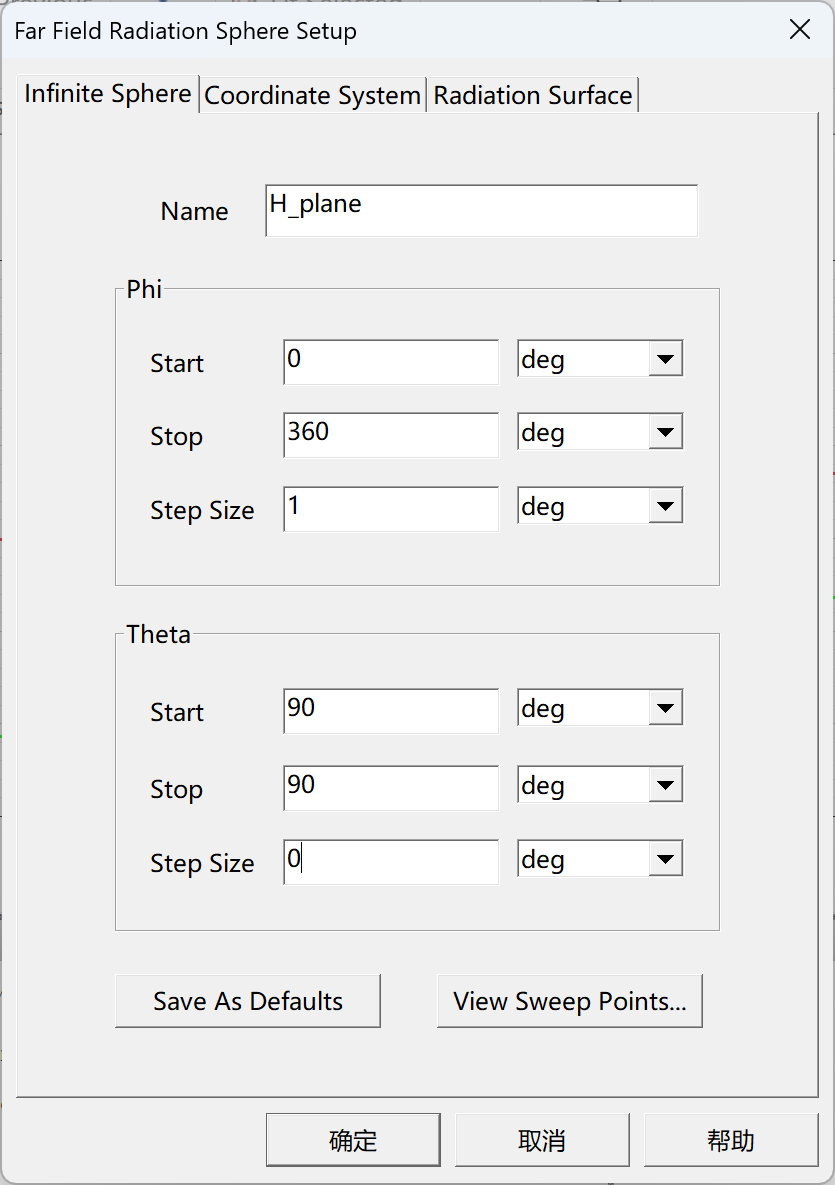
\includegraphics[width=0.32\textwidth]{p32.png}
             
        }%
            \subcaptionbox{3D-Sphere设置}[0.33\textwidth][c]{
            \centering
            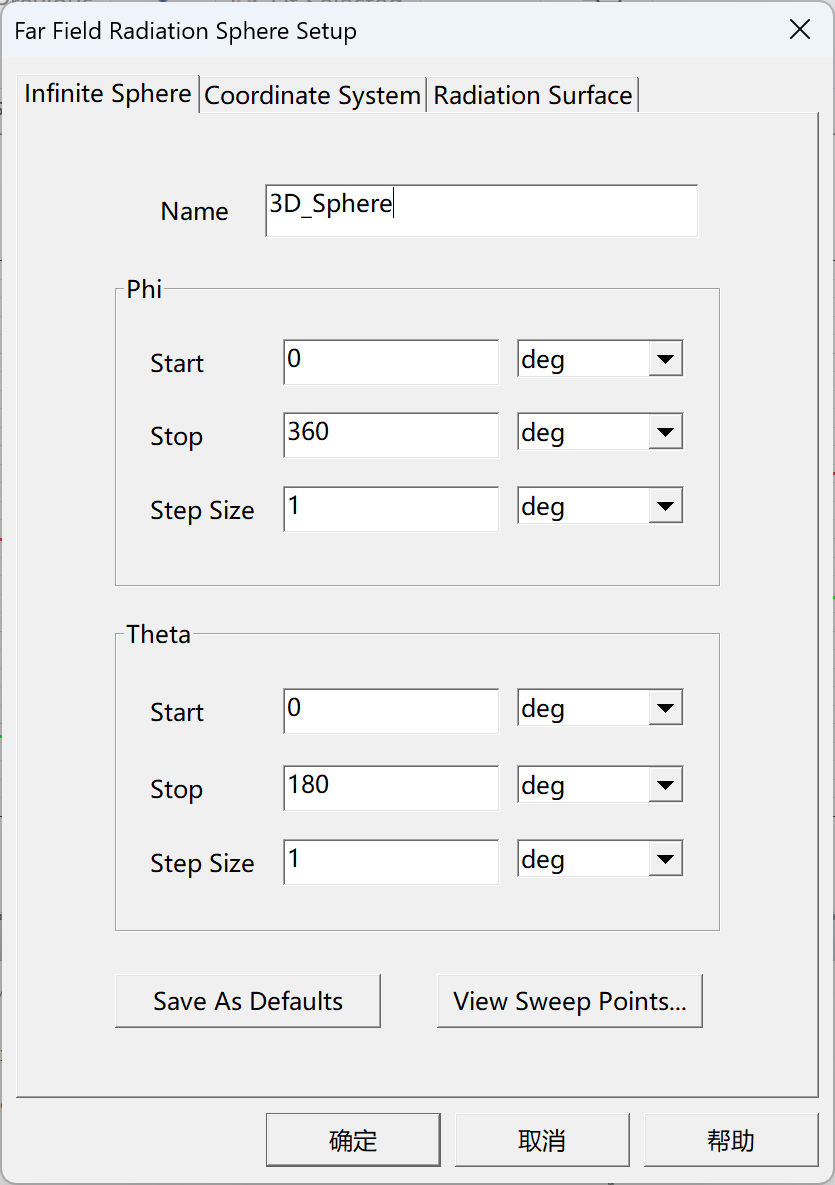
\includegraphics[width=0.32\textwidth]{p33.png}
             
        }%
        \caption{辐射表面设置}
         
    \end{figure}

（2）右键单击工程树下的\keyblue{Results}节点，在弹出的菜单中选择\keyblue{Create Far Fields Report}—\keyblue{Radiation Pattern}命令，如下设置对话框：

\begin{figure}[H]
    \centering
    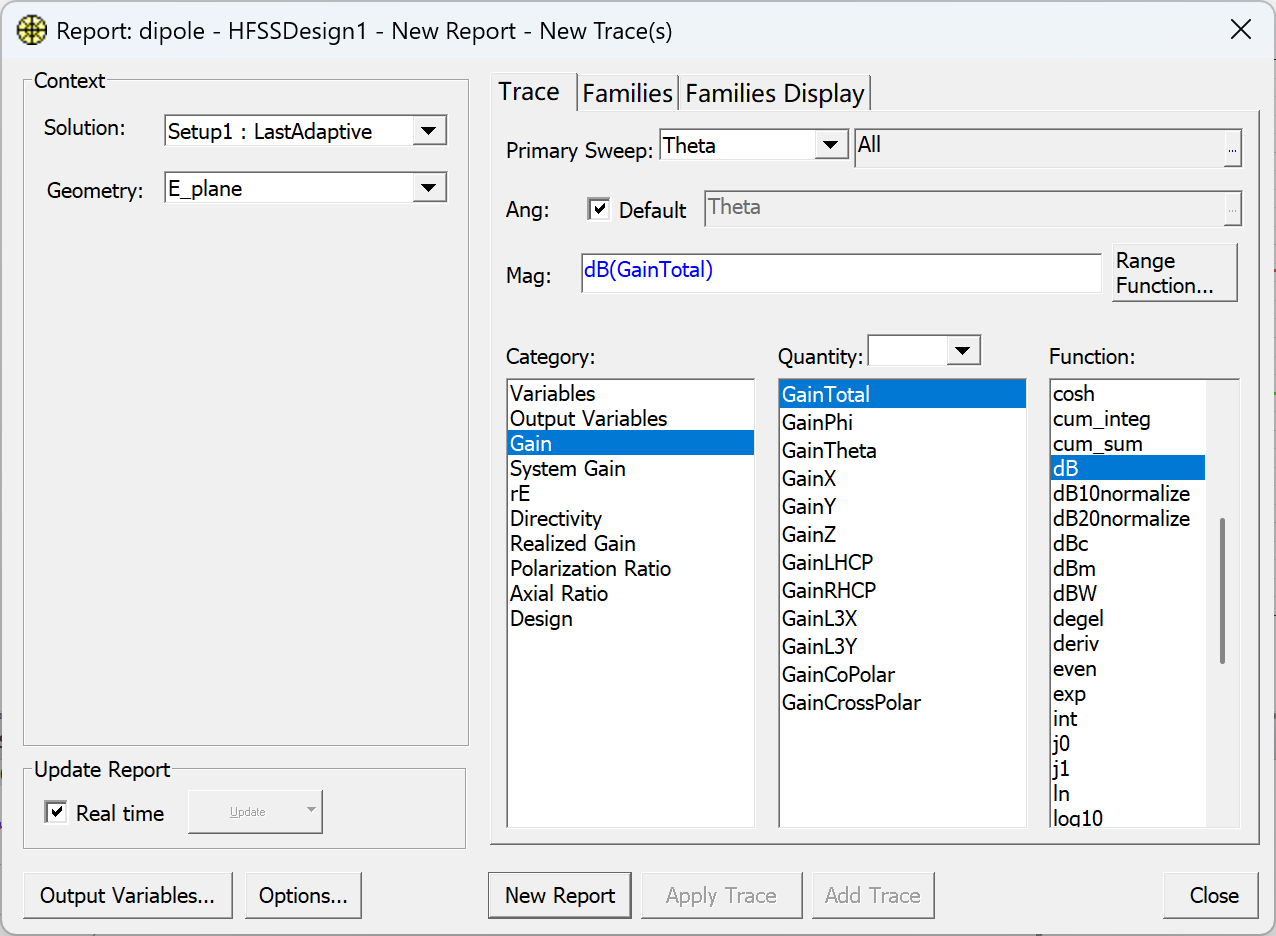
\includegraphics[width=0.8\textwidth]{p34.png}
    \caption{xz面方向图报告设置}
\end{figure}

点击\keyblue{New Report}按钮，生成极坐标系下天线的 xz 面增益方向图，如图所示：

\begin{figure}[H]
    \centering
    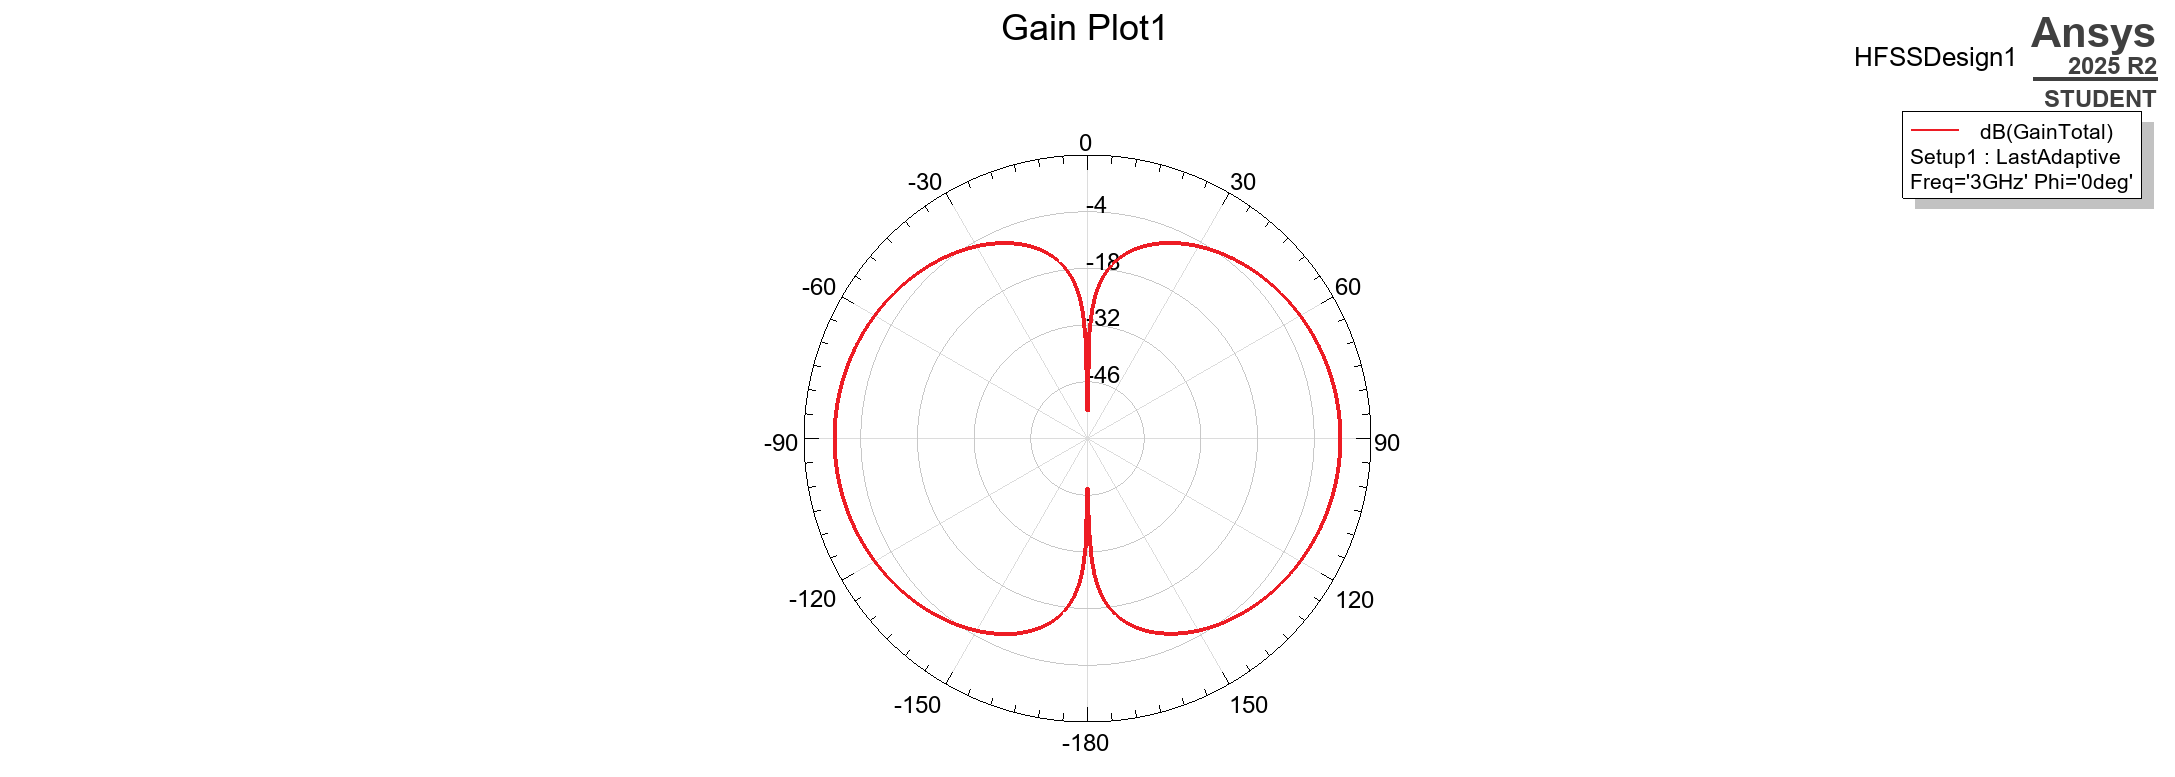
\includegraphics[width=0.8\textwidth]{p35.png}
    \caption{xz面增益方向图}
\end{figure}

【实验结果】:由图可知，在 $\phi = 0^{\circ}$ 时，
方向图呈现典型的“8”字形，
最大辐射方向位于垂直于天线轴线的$\theta=90^{\circ}$，
在天线轴线方向（$\theta=0^{\circ}$和 $\theta=180^{\circ}$）出现辐射零点。
仿真得到的最大增益约为 2.20 dB。

（3）右键单击工程树下的\keyblue{Results}节点，在弹出的菜单中选择\keyblue{Create Far Fields Report}—\keyblue{Radiation Pattern}命令，如下设置对话框：

\begin{figure}[H]
    \centering
    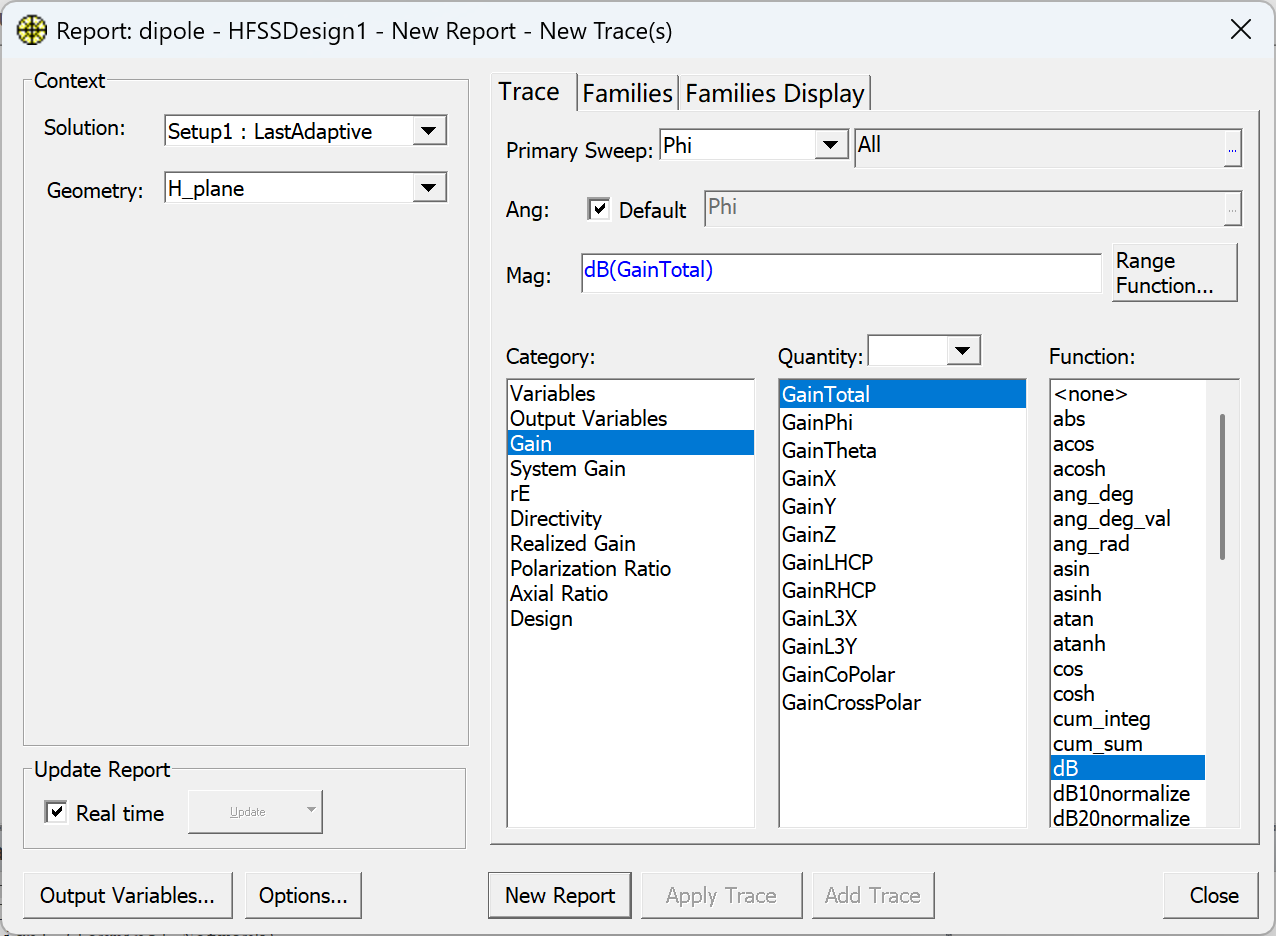
\includegraphics[width=0.8\textwidth]{p36.png}
    \caption{xy面方向图报告设置}
\end{figure}

点击\keyblue{New Report}按钮，生成天线的 xy 面增益方向图，如图所示：

\begin{figure}[H]
    \centering
    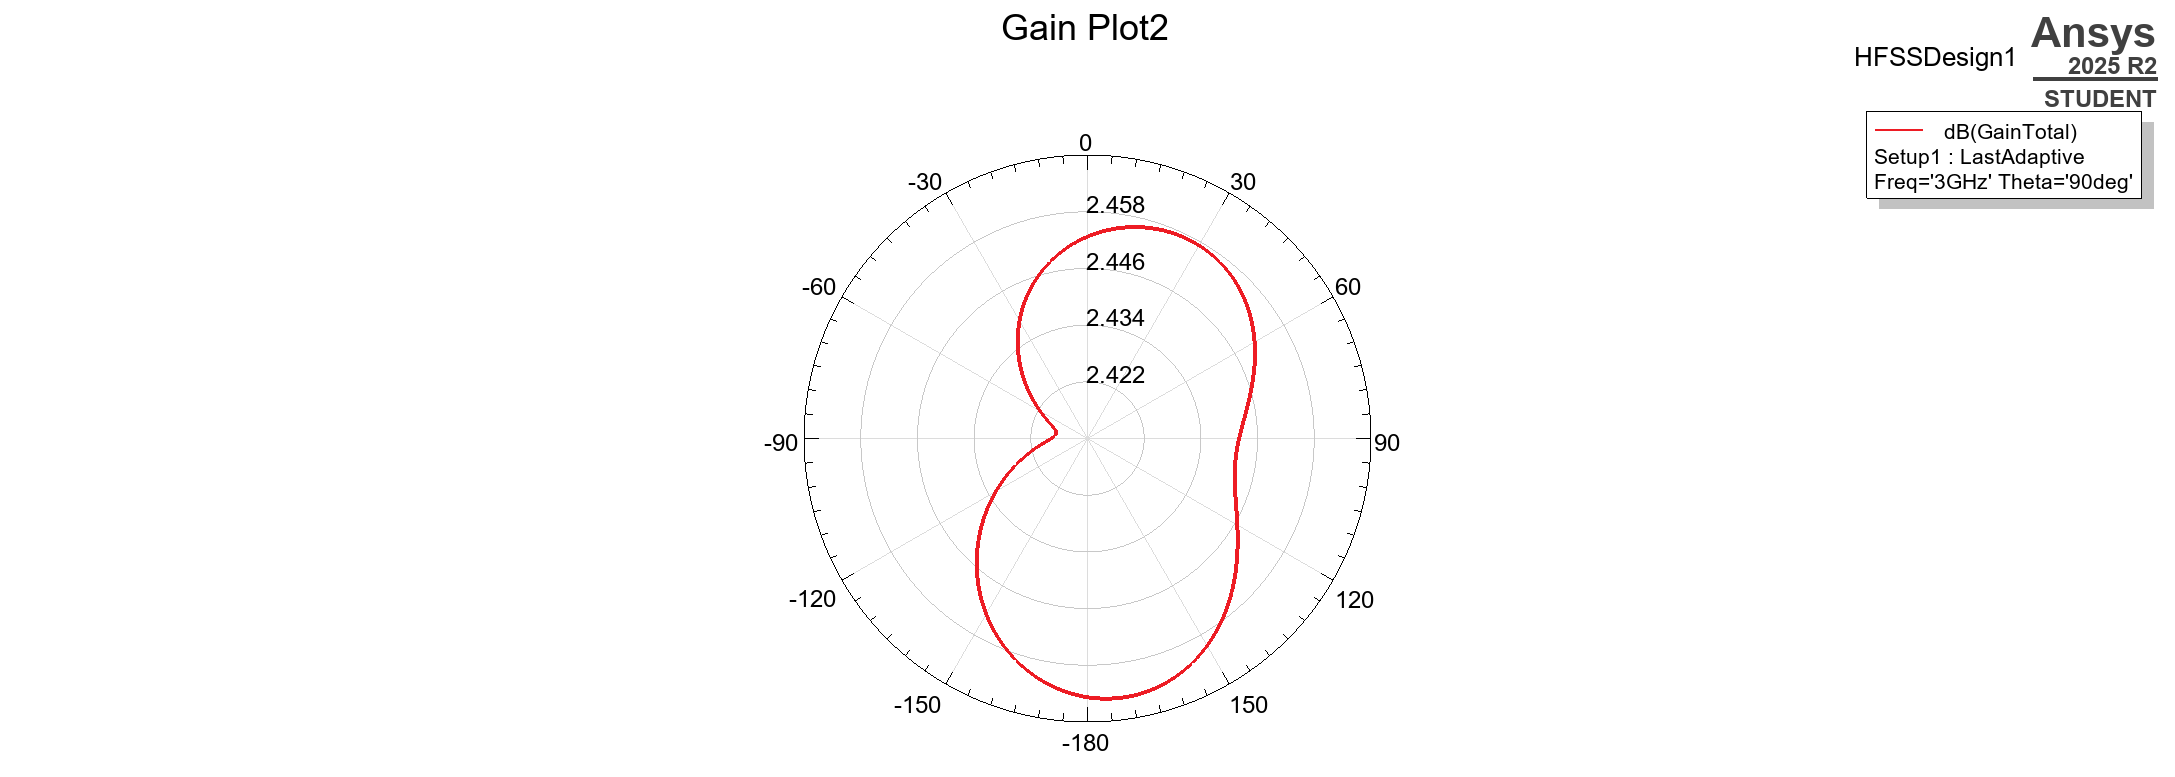
\includegraphics[width=0.8\textwidth]{p37.png}
    \caption{xy面增益方向图}
\end{figure}

【实验结果】:该方向图近似为圆形，表明天线在该平面内具有良好的全向辐射特性，增益变化平稳，约为 2.42 dB 左右

（4）右键单击工程树下的\keyblue{Results}节点，在弹出的菜单中选择\keyblue{Create Far Fields Report}—\keyblue{3D Polar Plot}命令，如下设置对话框：

\begin{figure}[H]
    \centering
    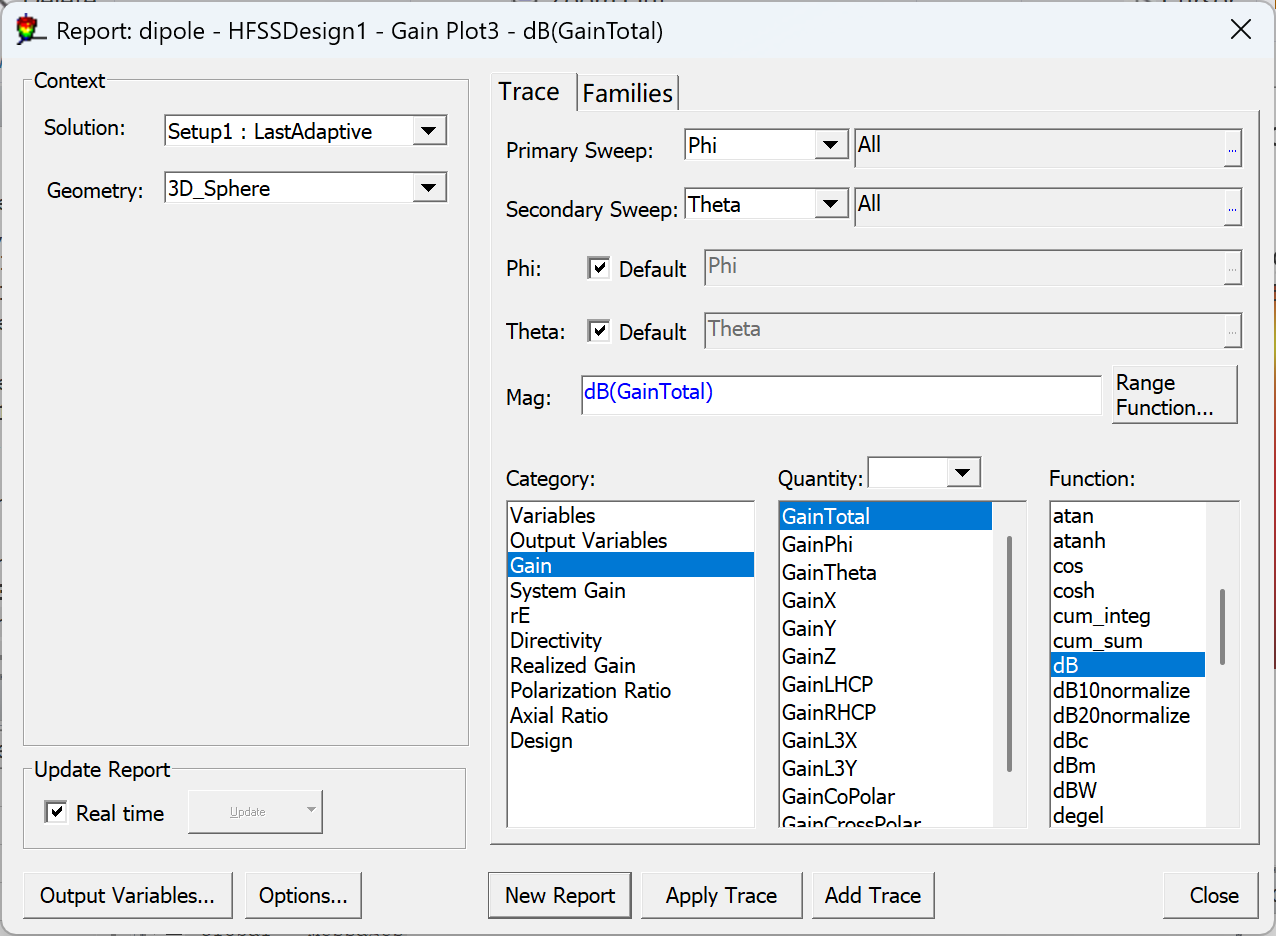
\includegraphics[width=0.8\textwidth]{p38.png}
    \caption{3D方向图报告设置}
\end{figure}

点击\keyblue{New Report}按钮，生成如下结果：

\begin{figure}[H]
    \centering
    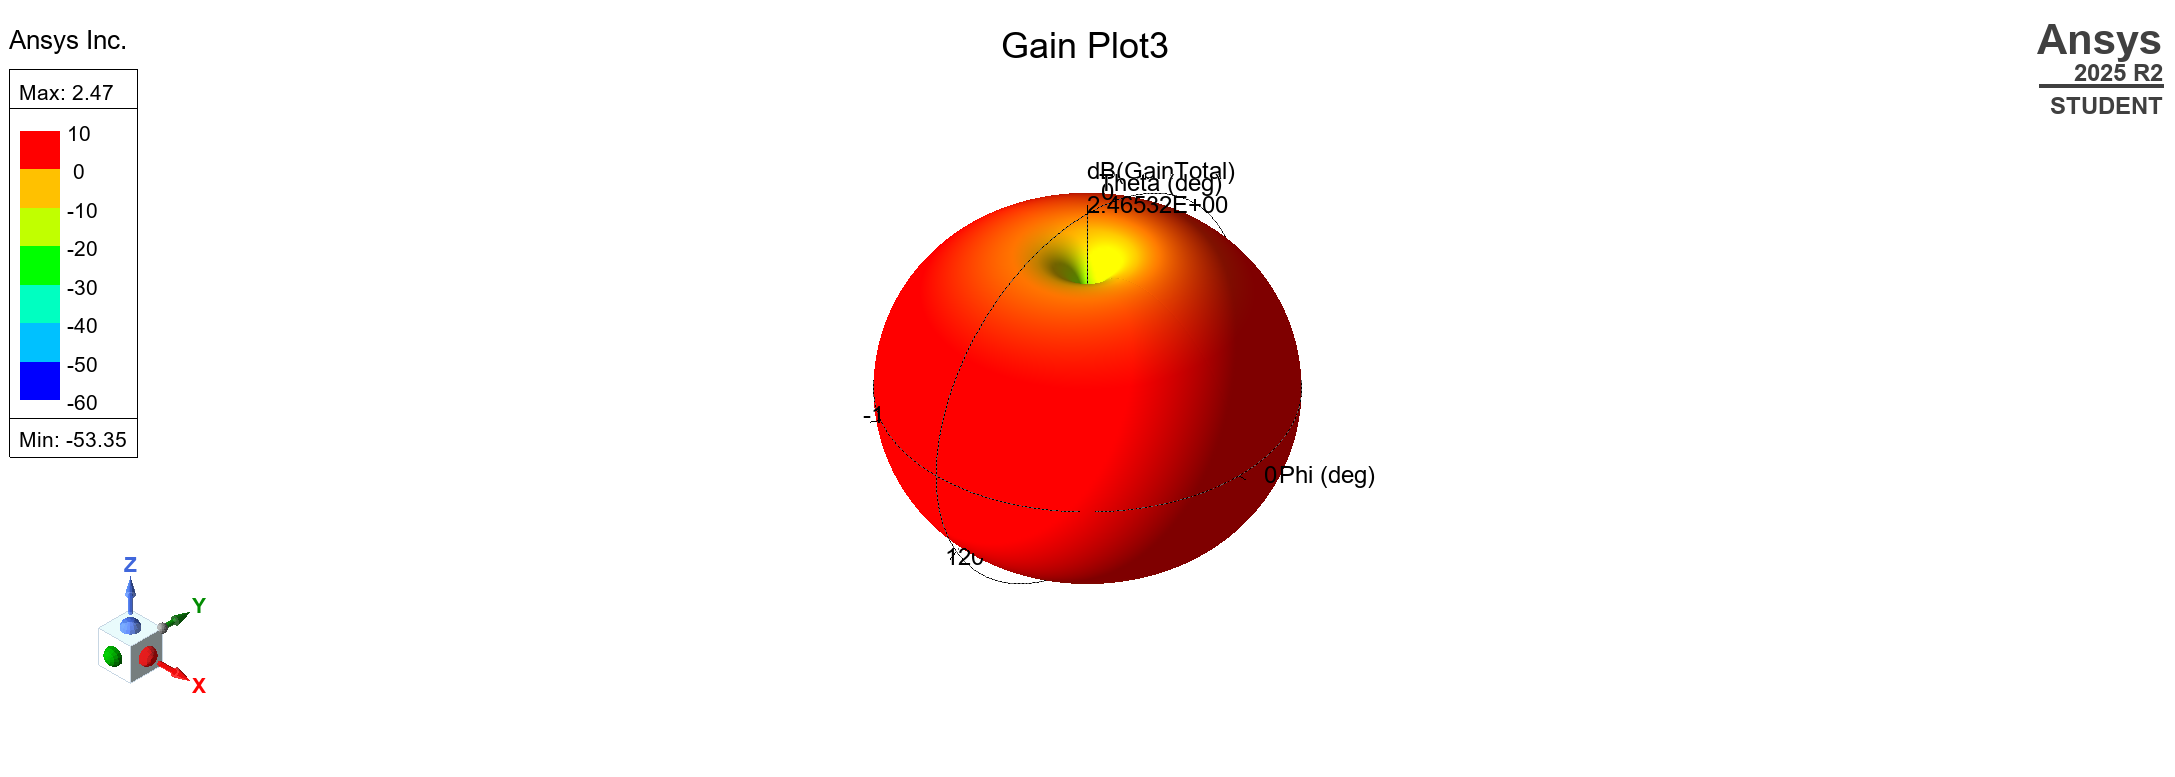
\includegraphics[width=0.8\textwidth]{p39.png}
    \caption{3D增益方向图}
\end{figure}

【实验结果】:由图可知，天线辐射能量集中在垂直于其轴线的平面，呈现标准的全向天线环形（甜甜圈形）辐射模式。最大增益为 2.47 dBi，方向与理论分析一致。 

\subsection{\heiti\bfseries 其他参数}

展开工程树下的\keyblue{Radiation}节点，右键单击\keyblue{3D Sphere}，在弹出的菜单中选择\keyblue{Compute Antenna Parameters}命令，可以得到天线在该辐射表面上的最大辐射强度、方向性系数、最大场强及其所在方向等参数，如图所示：

\begin{figure}[H]
    \centering
    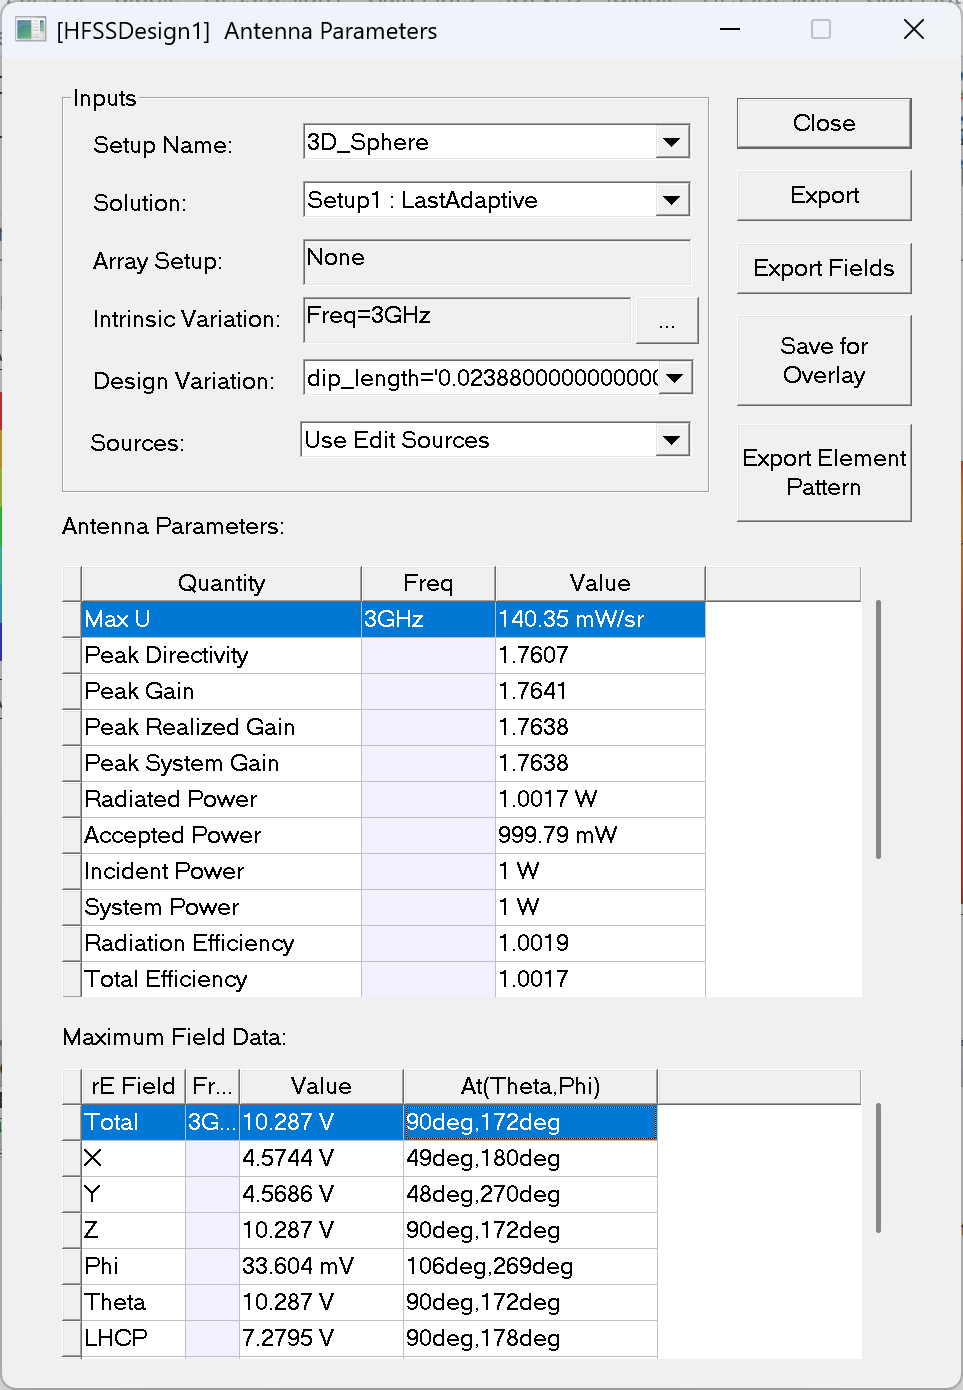
\includegraphics[width=0.8\textwidth]{p41.png}
    \caption{其他参数示意图}
\end{figure}

【实验结果】:由图可知，半波偶极子天线在工作频率 $3GHz$ 时的峰值方向性系数为 $1.7607$，峰值增益为 $1.7641$。
仿真结果中的效率略高于 100\%，这或许是由于计算精度产生的数值误差，但表明天线的辐射效率和总效率均非常接近理想值 100\%。

\section{\heiti\bfseries 实验总结与心得体会}

通过本次HFSS半波偶极子天线设计与仿真实验，我对天线的基本理论、设计方法和仿真技术有了更加深入的理解和掌握，主要收获和体会如下：

\subsection{\heiti\bfseries 理论与实践的结合}

本次实验让我深刻体会到理论知识与工程实践相结合的重要性。在实验前，我们学习了半波偶极子天线的电流分布、辐射场、方向性系数等理论知识，通过HFSS仿真，实际得到的辐射电阻、方向性系数等参数与理论值高度吻合，验证了理论分析的正确性。这种理论与仿真相互印证的过程，加深了我对天线工作原理的理解。

\subsection{\heiti\bfseries HFSS软件操作能力的提升}

通过本次实验，我系统学习并掌握了HFSS软件的基本操作流程，包括：

\begin{itemize}
    \item 工程的创建与设置（求解类型选择、单位设置等）
    \item 参数化建模方法（通过定义变量实现模型的灵活调整）
    \item 三维模型的构建（圆柱体、矩形面等基本几何体的创建与操作）
    \item 边界条件和激励源的设置（辐射边界、集总端口等）
    \item 求解器配置（求解频率、网格剖分、扫频设置等）
    \item 后处理与结果分析（S参数、驻波比、Smith圆图、方向图等）
\end{itemize}

\subsection{\heiti\bfseries 实验中遇到的问题与解决}

在实验过程中，我也遇到了一些问题，通过询问助教和调试得以解决：

\begin{itemize}
    \item {\heiti\bfseries 软件配置}：初期在设置时遇到打开“Ansys Electronics Desktop Student 2025 R2“
自动跳转到“Ansys Twin Builder Student 2025 R2”的问题，通过询问助教更改Config为All后顺利解决
    
    \item {\heiti\bfseries 单位设置}：第一次建模时忘记将单位设置为mm，导致模型尺寸过大，仿真停滞不前，通过重新设置单位并调整模型尺寸解决。
    \end{itemize}

\subsection{\heiti\bfseries 总结}
实验结果表明，设计的半波偶极子天线各项性能指标均符合预期，达到了实验目的。
通过本次实验，我不仅掌握了HFSS软件的基本操作，更重要的是培养了将理论知识应用于工程实践的能力。

\end{document}
